\documentclass[11pt,letterpaper]{exam}
\usepackage[spanish]{babel}
\usepackage{graphicx}
\usepackage{tabularx}
\usepackage[absolute]{textpos} % Para poner una imagen en posiciones arbitrarias
\usepackage{multirow}
\usepackage{float}
\usepackage{hyperref}
\usepackage[utf8x]{inputenc} 
\usepackage[normalem]{ulem}
\useunder{\uline}{\ul}{}
\usepackage[usenames]{color}
\title{Tarea 2 Metodos Computacionales}
\author{Valeria Martin Hernandez}

\date{Mayo 2019}

\begin{document}


\maketitle
\newpage


\section{Ejercicio 2: Transformadas de Fourier}

\subsection{Signal.dat y signalSuma.dat:}
\subsubsection{Grafica general}
\begin{figure}[H]
    \centering
    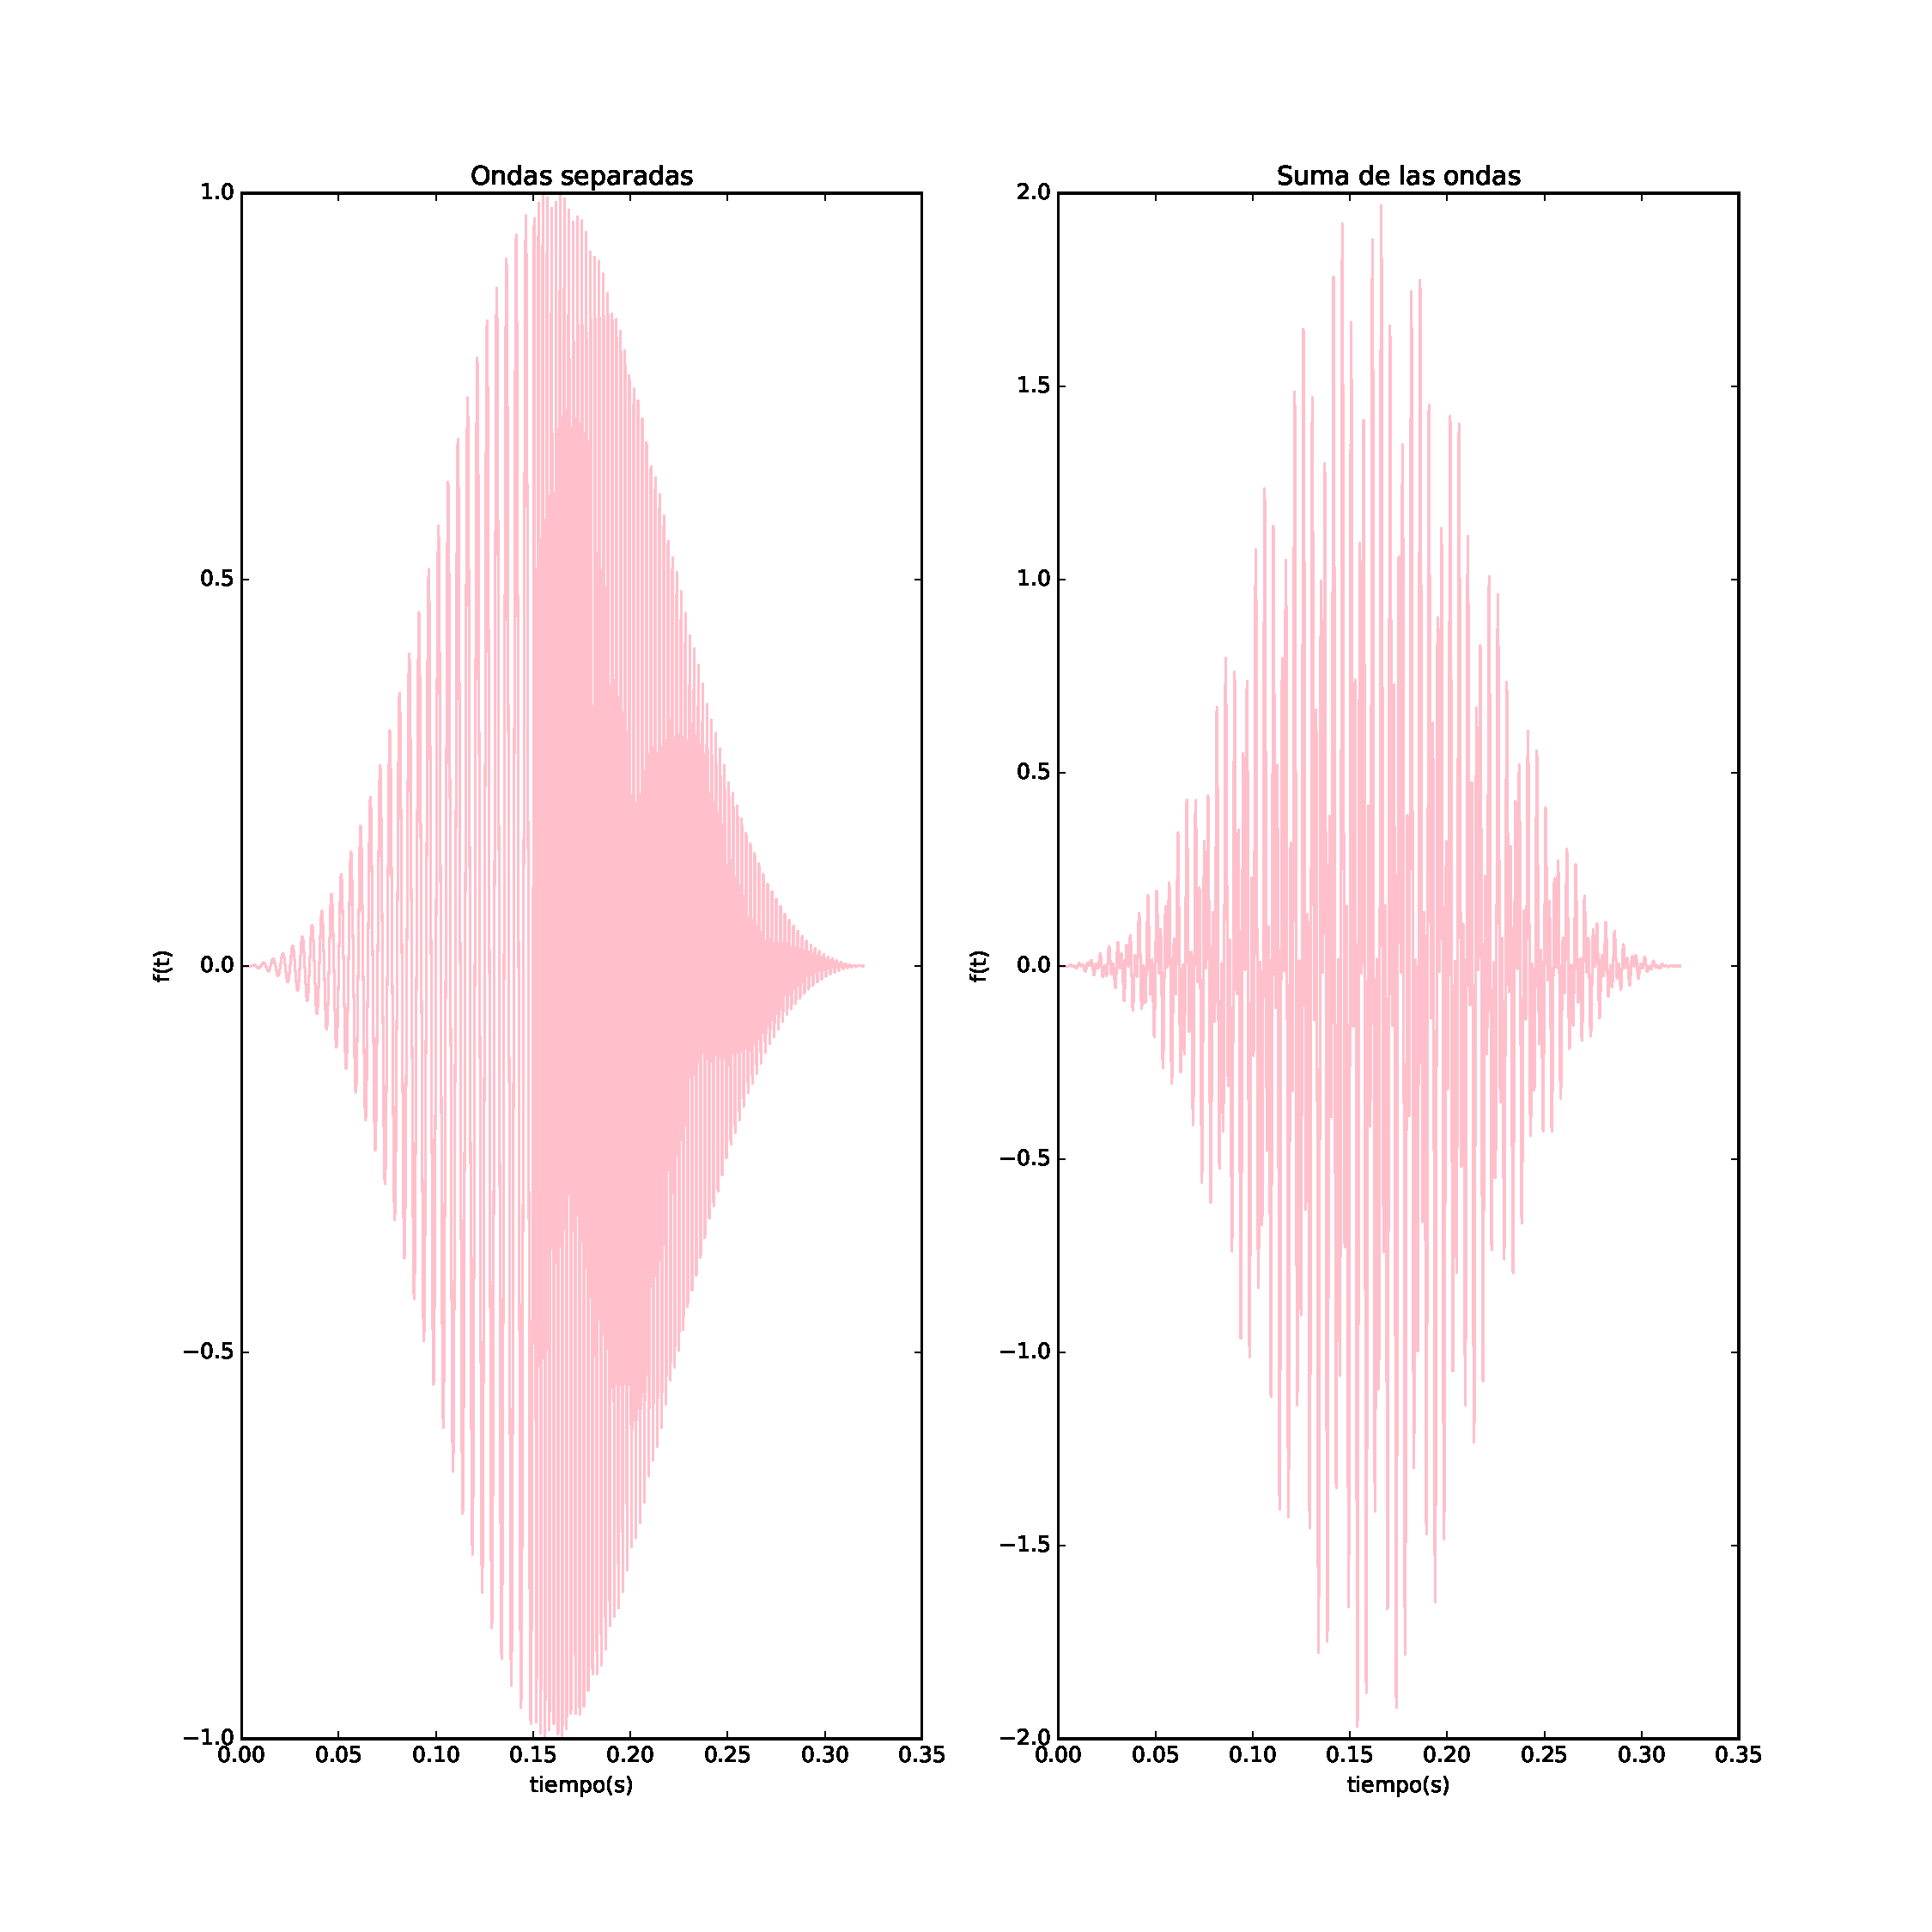
\includegraphics[width=1\textwidth]{signals.pdf}
    \caption{Grafica de las seniales.}
    \label{fig:my_label}
\end{figure}

En esta grafica se observan dos representaciones de dos ondas, la primera esta conformada por dos seniales, primero una y despues la otra y la segunda es la suma de estas dos seniales. Se observa que las graficas cambian bastante, ya que en la primera grafica se tiene una curva mucho mas suave, mientras que en la segunda hay una mayor cantidad de picos. Esto seguramente se debe a que la suma de las graficas hace que se disminuyan los valores en el eje y. Por otro lado, se observa, en la imagen de la izquierda, que una de las ondas tiene un periodo mucho mayor en comparacion a la otra. En efecto, se ve una saturacion mayor en la parte derecha de esta grafica. Sin embargo, como se puede en la grafica izquierda, ambas ondas son bastante parecidas.

\subsubsection{Grafica de la transforma de fourier para las seniales}
\begin{figure}[H]
    \centering
    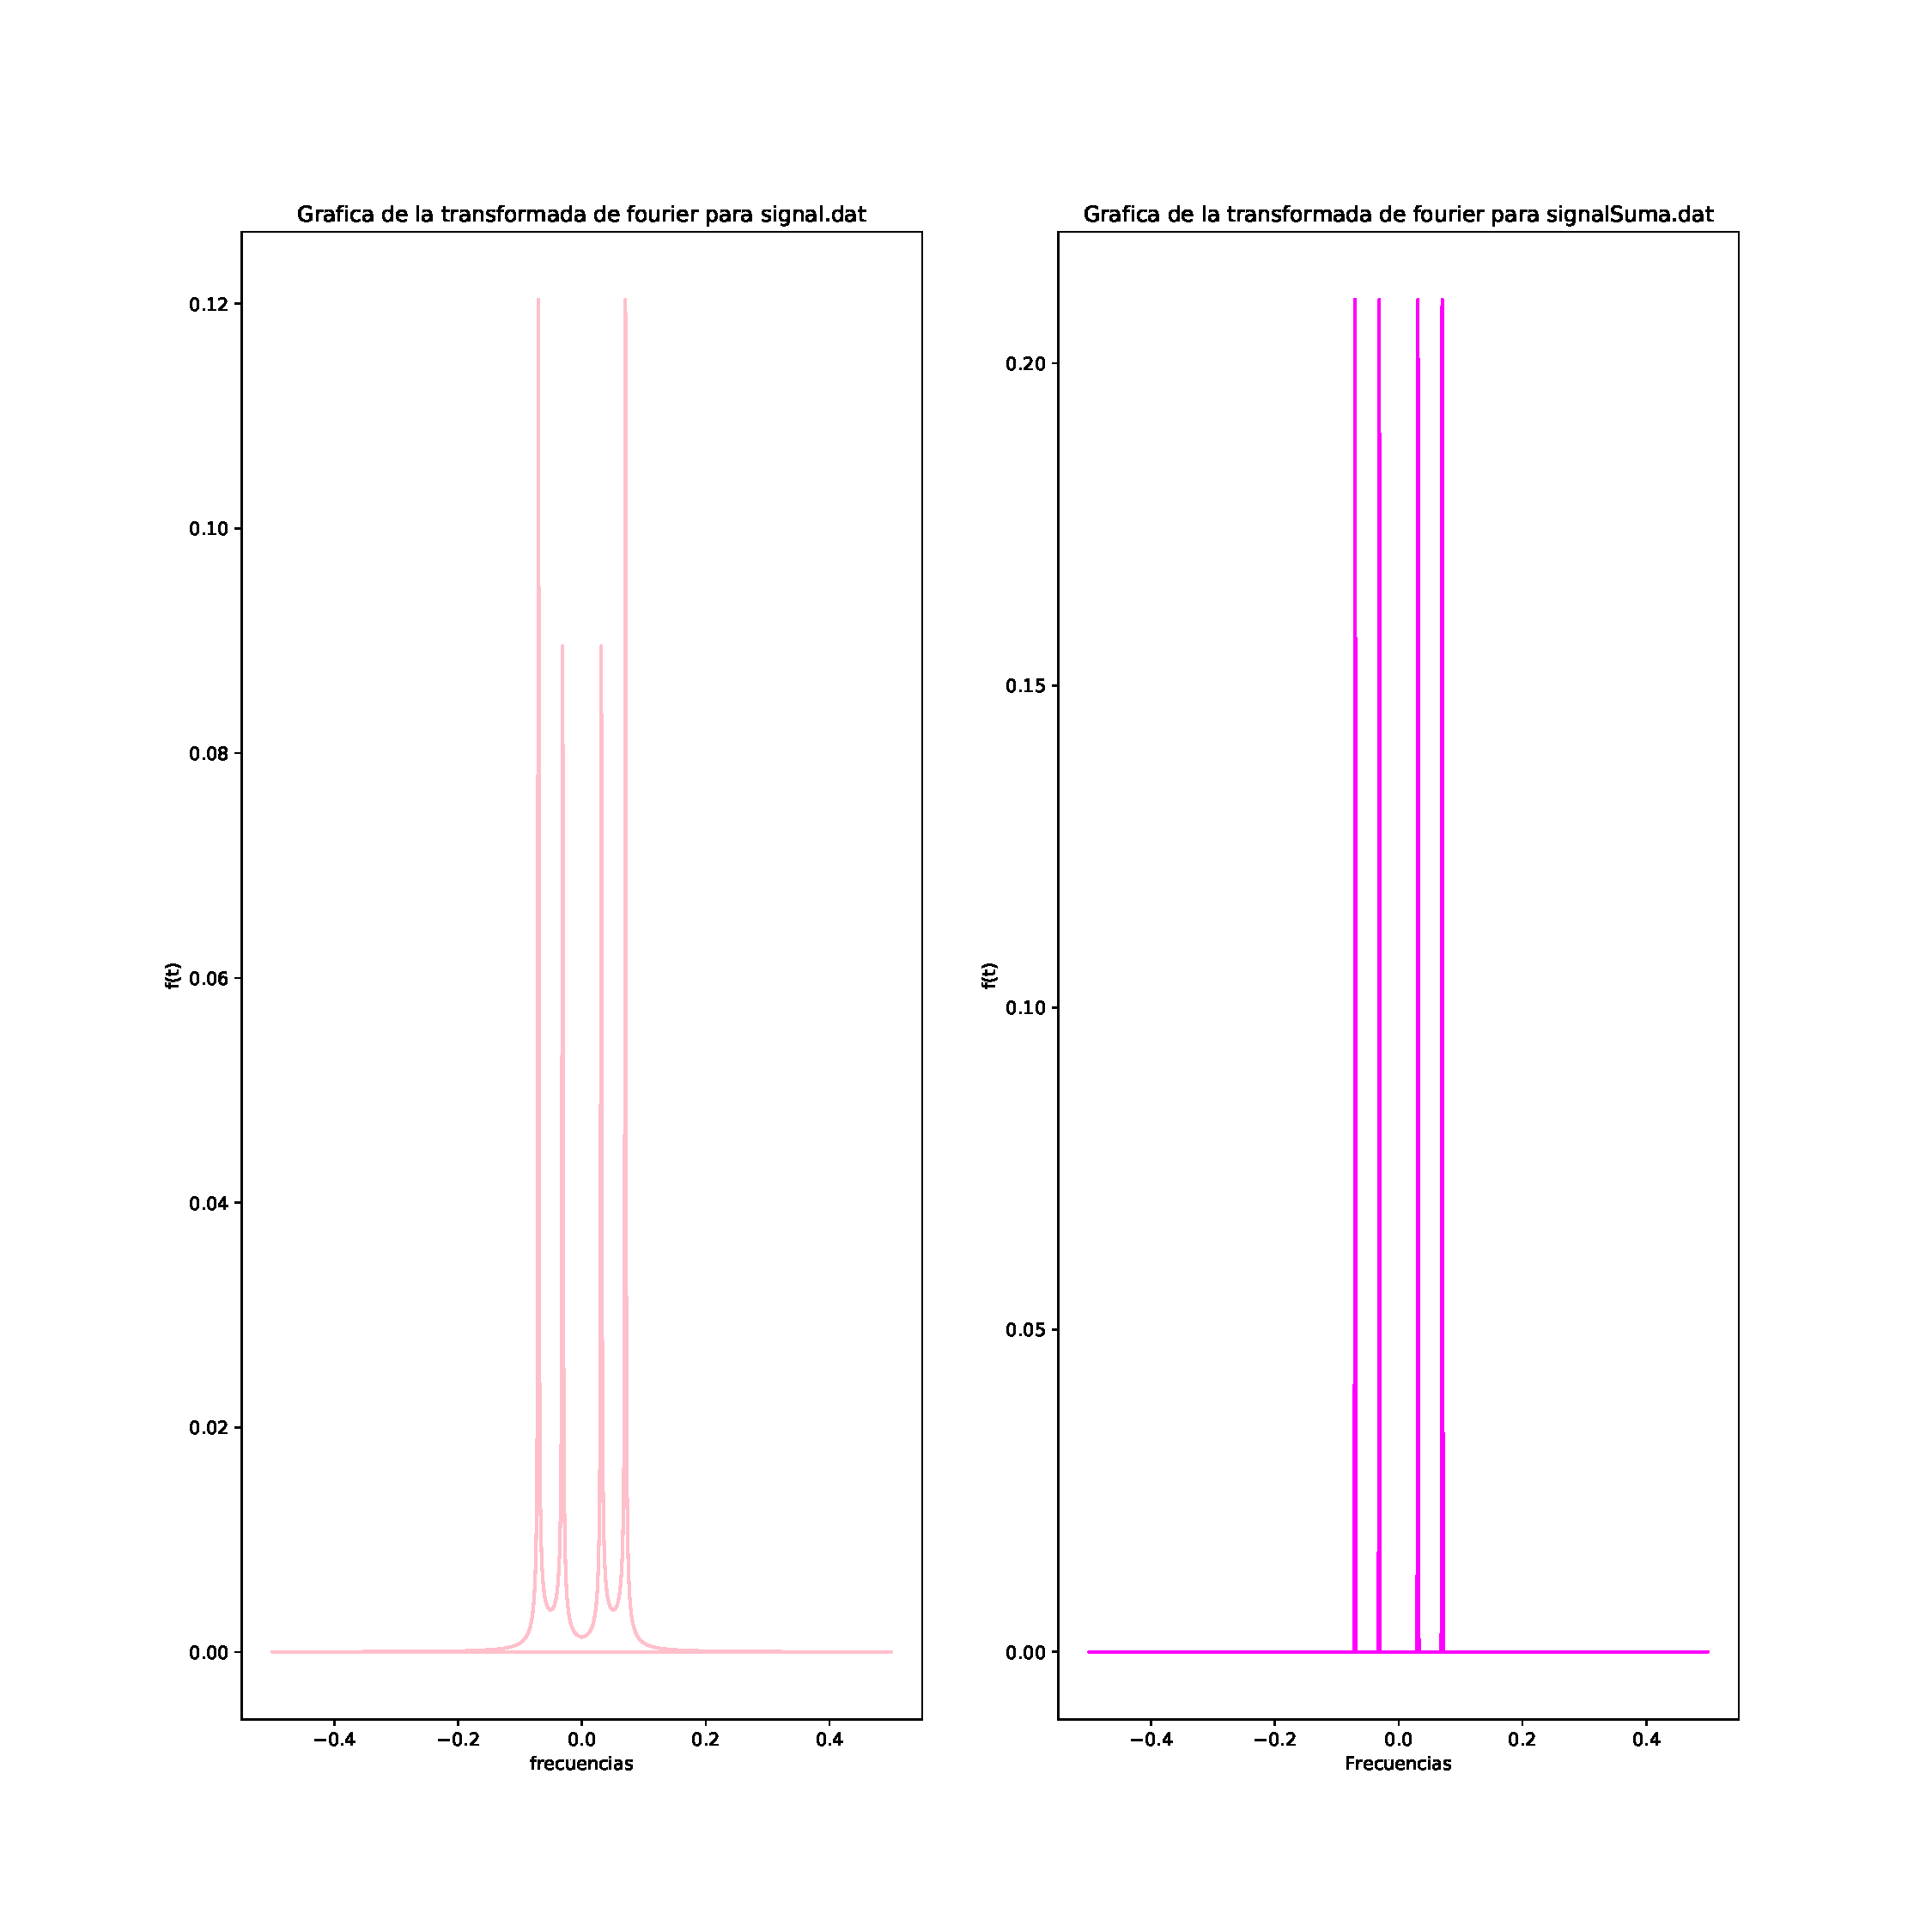
\includegraphics[width=1\textwidth]{Fourier_trans.pdf}
    \caption{Grafica de las transformadas de fourier para las dos primeras seniales.}
    \label{fig:my_label}
\end{figure}
En esta grafica se tiene de la transformada de fourier para ambas seniales en funcion de las frecuencias. Se observa que ambas curvas son sumamente parecidas. De hecho, las frecuencias principales coinciden. Se determino que los valores mas importantes de la transformada se encuentran en las frecuencias de -450 y 450. Ahora bien, la transformada de Fourier suele utilizarse para tener datos en el dominio de las frecuencias. En este caso, la grafica nos permite entender donde se concentran las energias de las diferentes seniales.  Esto quiere decir que se espera tener altas energias en las frecuencias mencionadas anteriormente.
\subsubsection{Espectograma}
\begin{figure}[H]
    \centering
    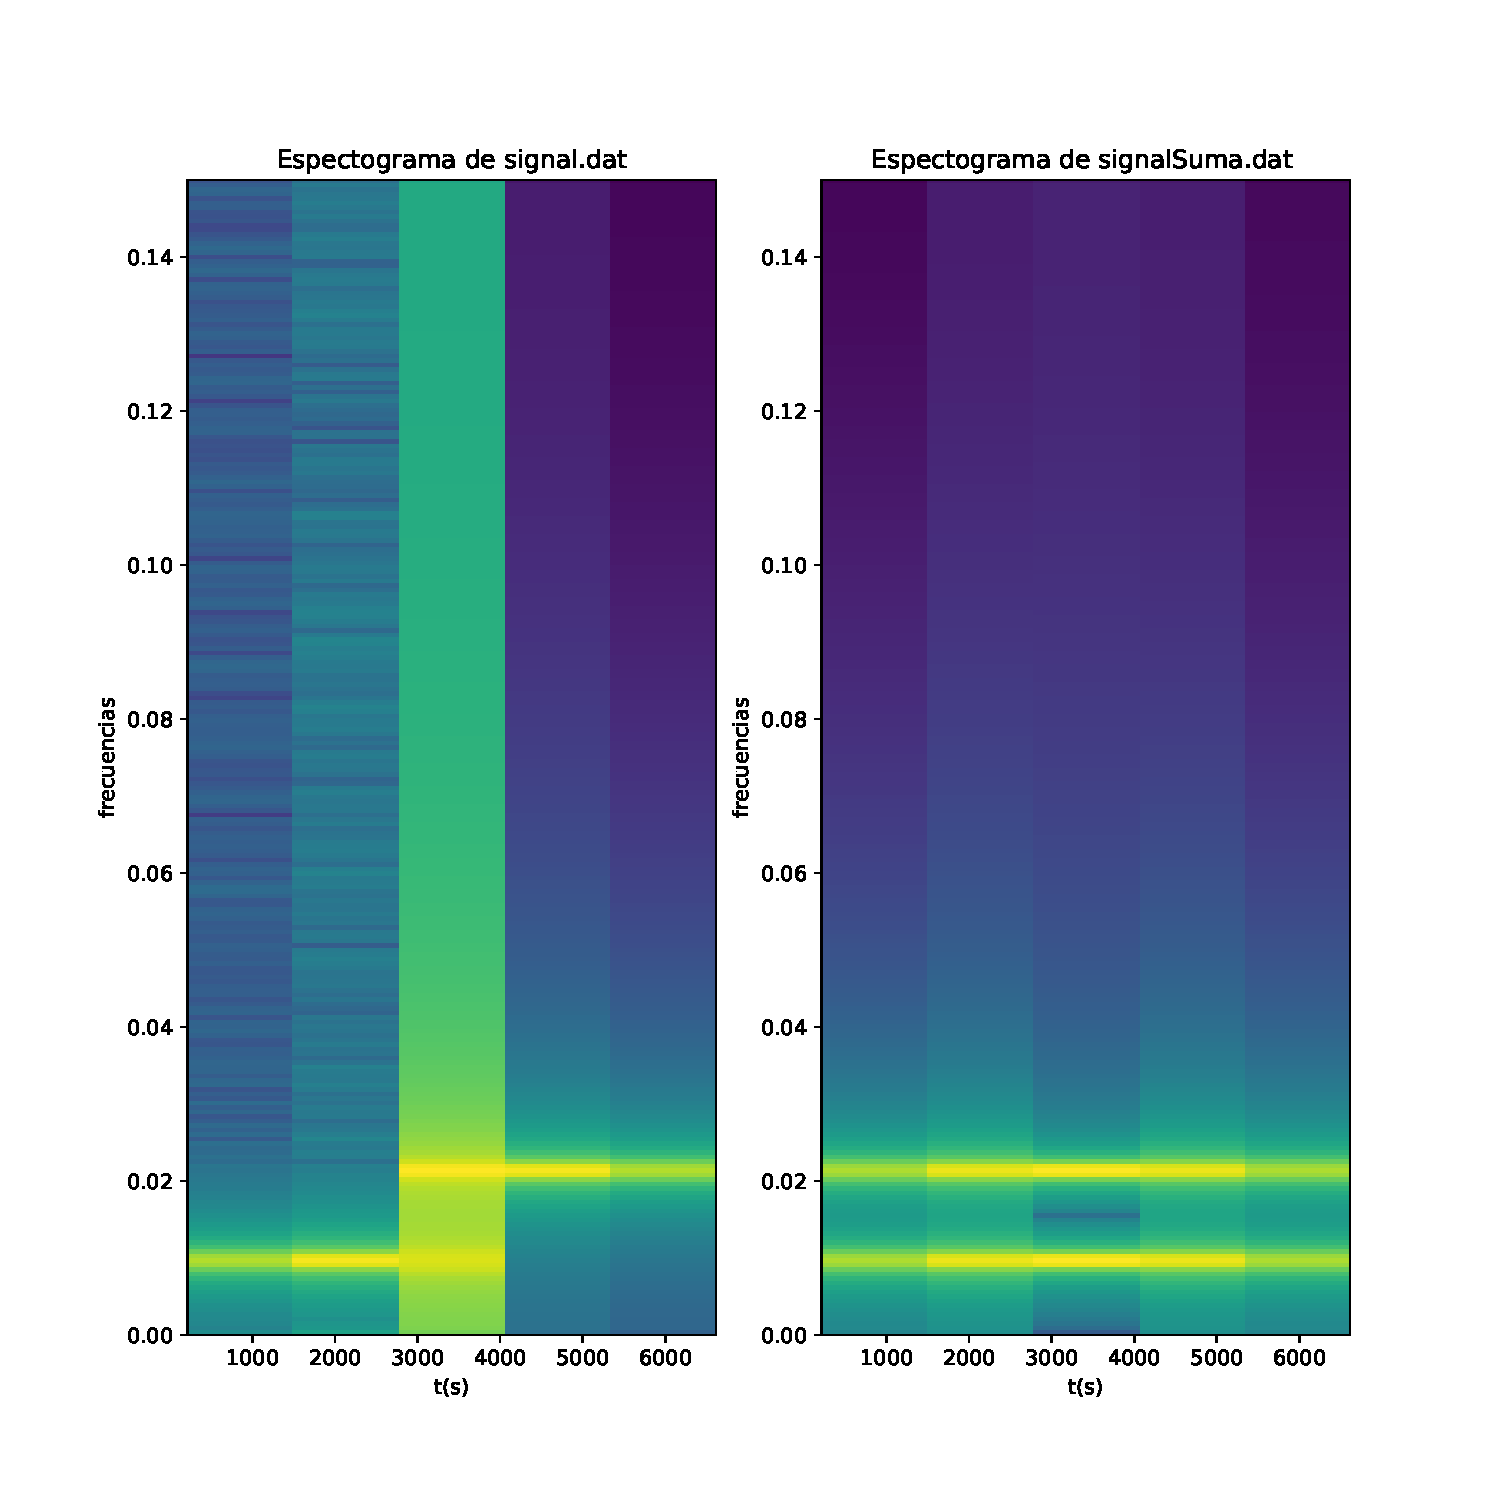
\includegraphics[width=1\textwidth]{espectograma.pdf}
    \caption{Espectogramas de las dos primeras seniales.}
    \label{fig:my_label}
\end{figure}
Estos espectogramas nos muestran resultados bastante similares a lo visto en la figura 2. En efecto, se ve que coinciden bastante ambas graficas con lo que se obtuvo al plottear las transformadas de fourier. Esto nos indica que los espectogramas son una representacion de la transformada de fourier en funcion de las frecuencias. Tambien, estos espectogramas nos permiten visualizar la fuerza y la energia que posee la senial a traves del tiempo. Segun lo visto en la pagina web \url{https://pnsn.org/spectrograms/what-is-a-spectrogram} se observa que hay un cambio de energia entre las dos graficas. 
\subsection{Temblor.txt:}
\subsubsection{Grafica general}
\begin{figure}[H]
    \centering
    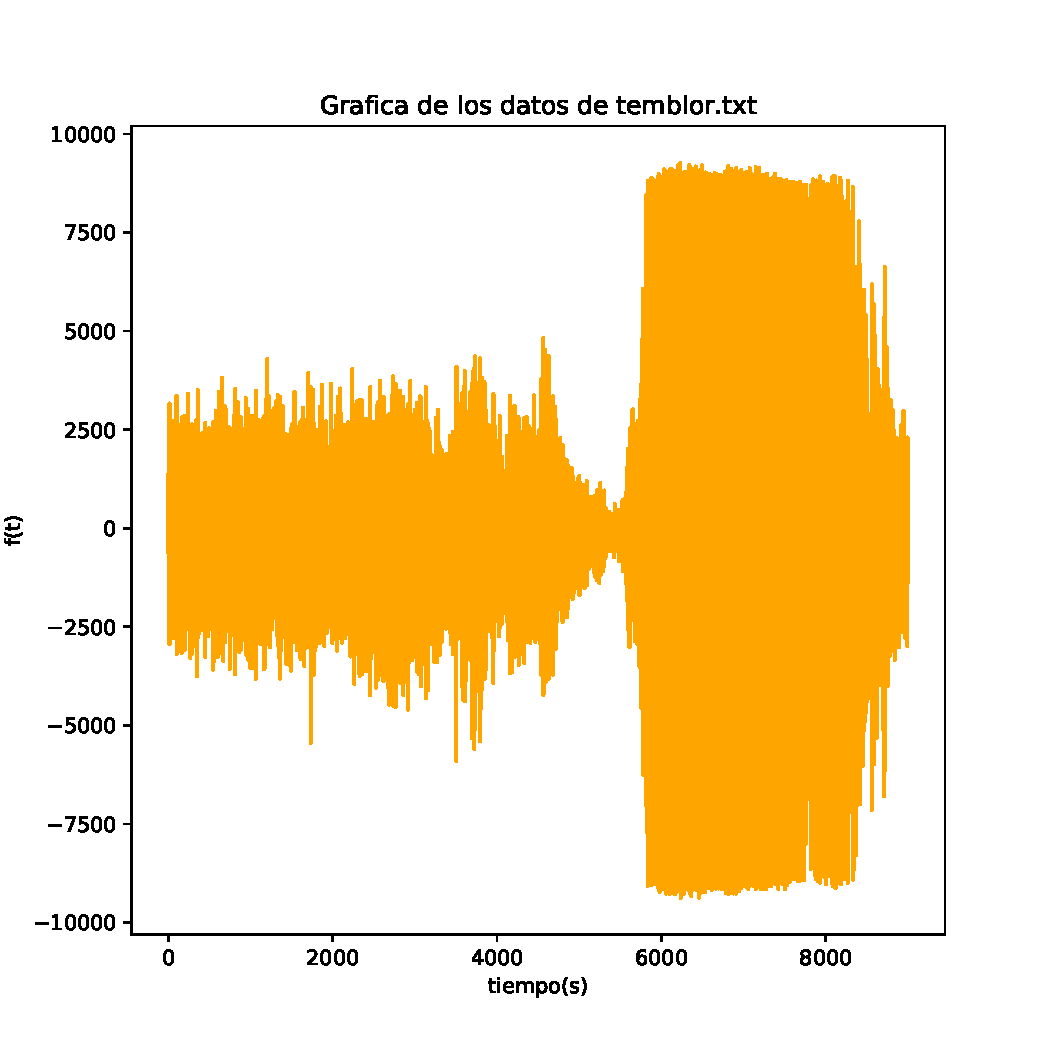
\includegraphics[width=1\textwidth]{Temblor.pdf}
    \caption{Grafica de los datos de temblor.txt}
    \label{fig:my_label}
\end{figure}
En esta grafica se observa la senial emitida por un temblor.En general se observa que hay una amplitud que rodea los valores de 2500 hasta los 4500 segundos. En los 4500 segundos este temblor se detiene y luego comienza uno con una fuerza mucho mayor. No se considera que esto se deba a una replica, ya que esto no explicaria el aumento en la amplitud de la senial. 
\subsubsection{Grafica transformada de fourier}
\begin{figure}[H]
    \centering
    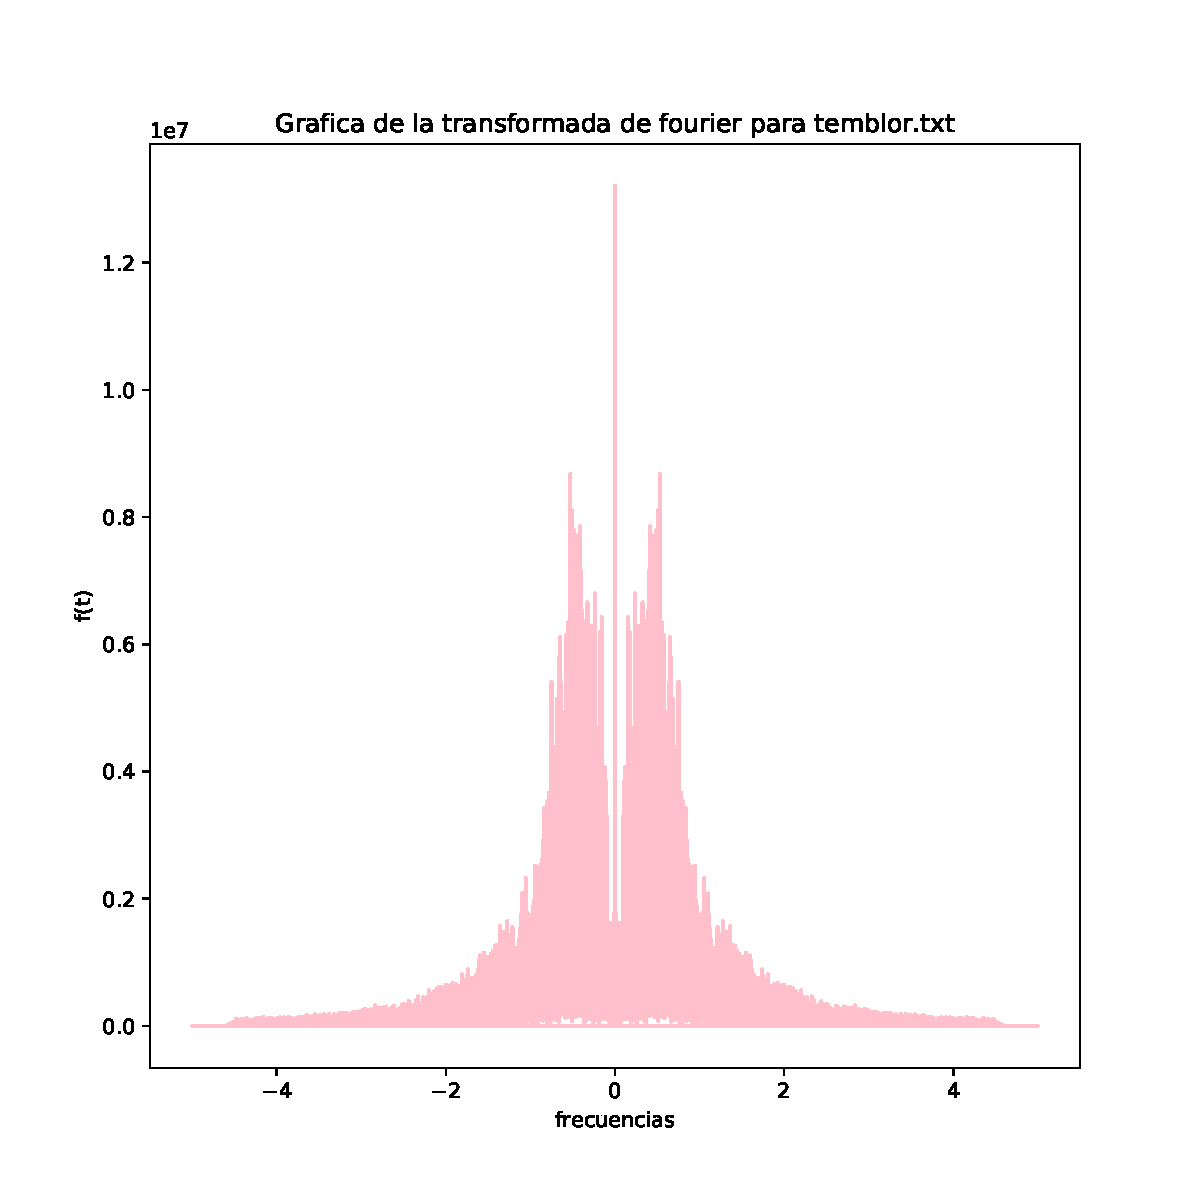
\includegraphics[width=1\textwidth]{Fourier_temblor.pdf}
    \caption{Grafica de las transformada de fourier de los datos de temblor.txt}
    \label{fig:my_label}

\end{figure}
En esta grafica se tiene la transformada de fourier en funcion de la frecuencia para los datos del temblor. Se observa que se obtiene el mayor valor de la transformada para una frecuencia de 0 y que hay otros dos valores importante para frecuencias de -0.1 y 0.1.Ahora bien, la transformada de Fourier suele utilizarse para tener datos en el dominio de las frecuencias. En este caso, la grafica nos permite entender donde se concentran las energias de las diferentes seniales.   Esto quiere decir que se espera tener altas energias en las frecuencias mencionadas anteriormente.
\subsubsection{Espectograma}
\begin{figure}[H]
    \centering
    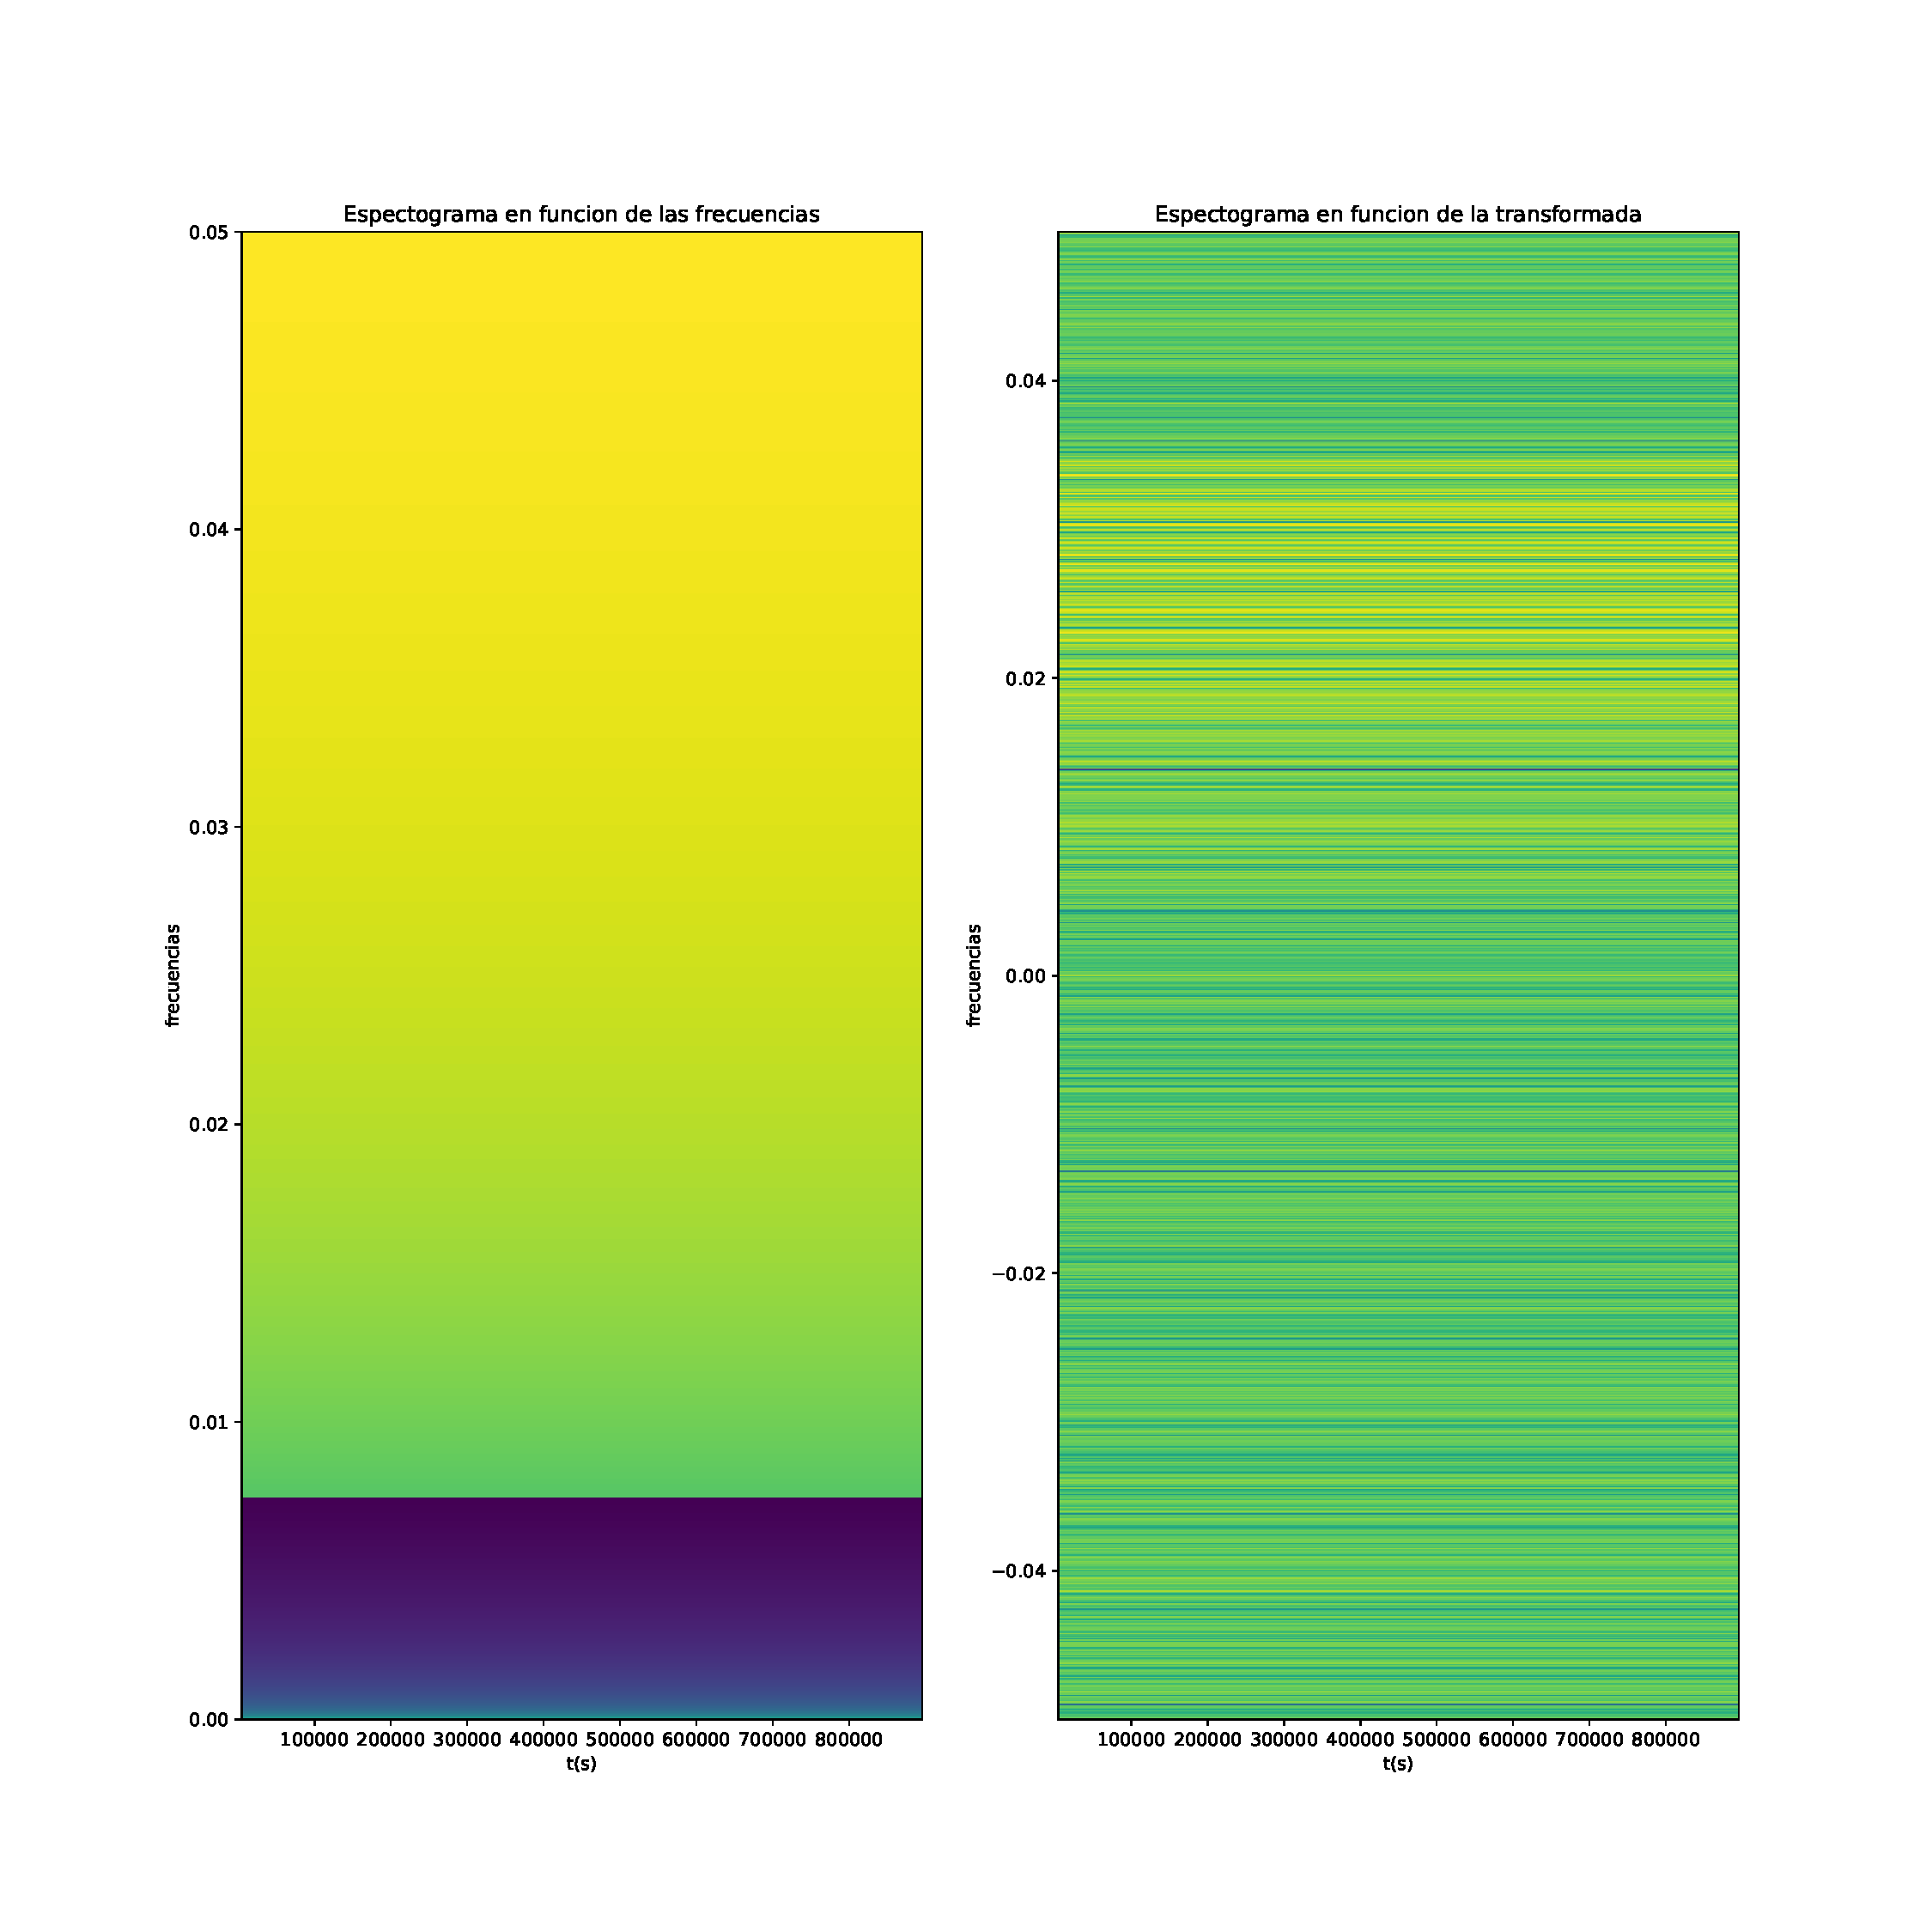
\includegraphics[width=1\textwidth]{espectograma_temblor.pdf}
    \caption{Espectograma del temblor}
    \label{fig:my_label}
\end{figure}
Una vez mas, este espectograma muestra similitudes con la grafica de la transformada de Fourier. Segun lo visto en la pagina weB \url{https://pnsn.org/spectrograms/what-is-a-spectrogram} se sabe que este espectograma corresponde a un temblor no volcanico. Ya que el cambio y la magnitud de las energias nos lo demuestra. Por otro lado, la energia aumenta bastante despues de 27000s, lo que nos indica un aumento en la fuerza del temblor.
\section{Ejercicio 2: Ecuaciones diferenciales ordinarias}
\subsection{Primera grafica}
\begin{figure}[H]
    \centering
    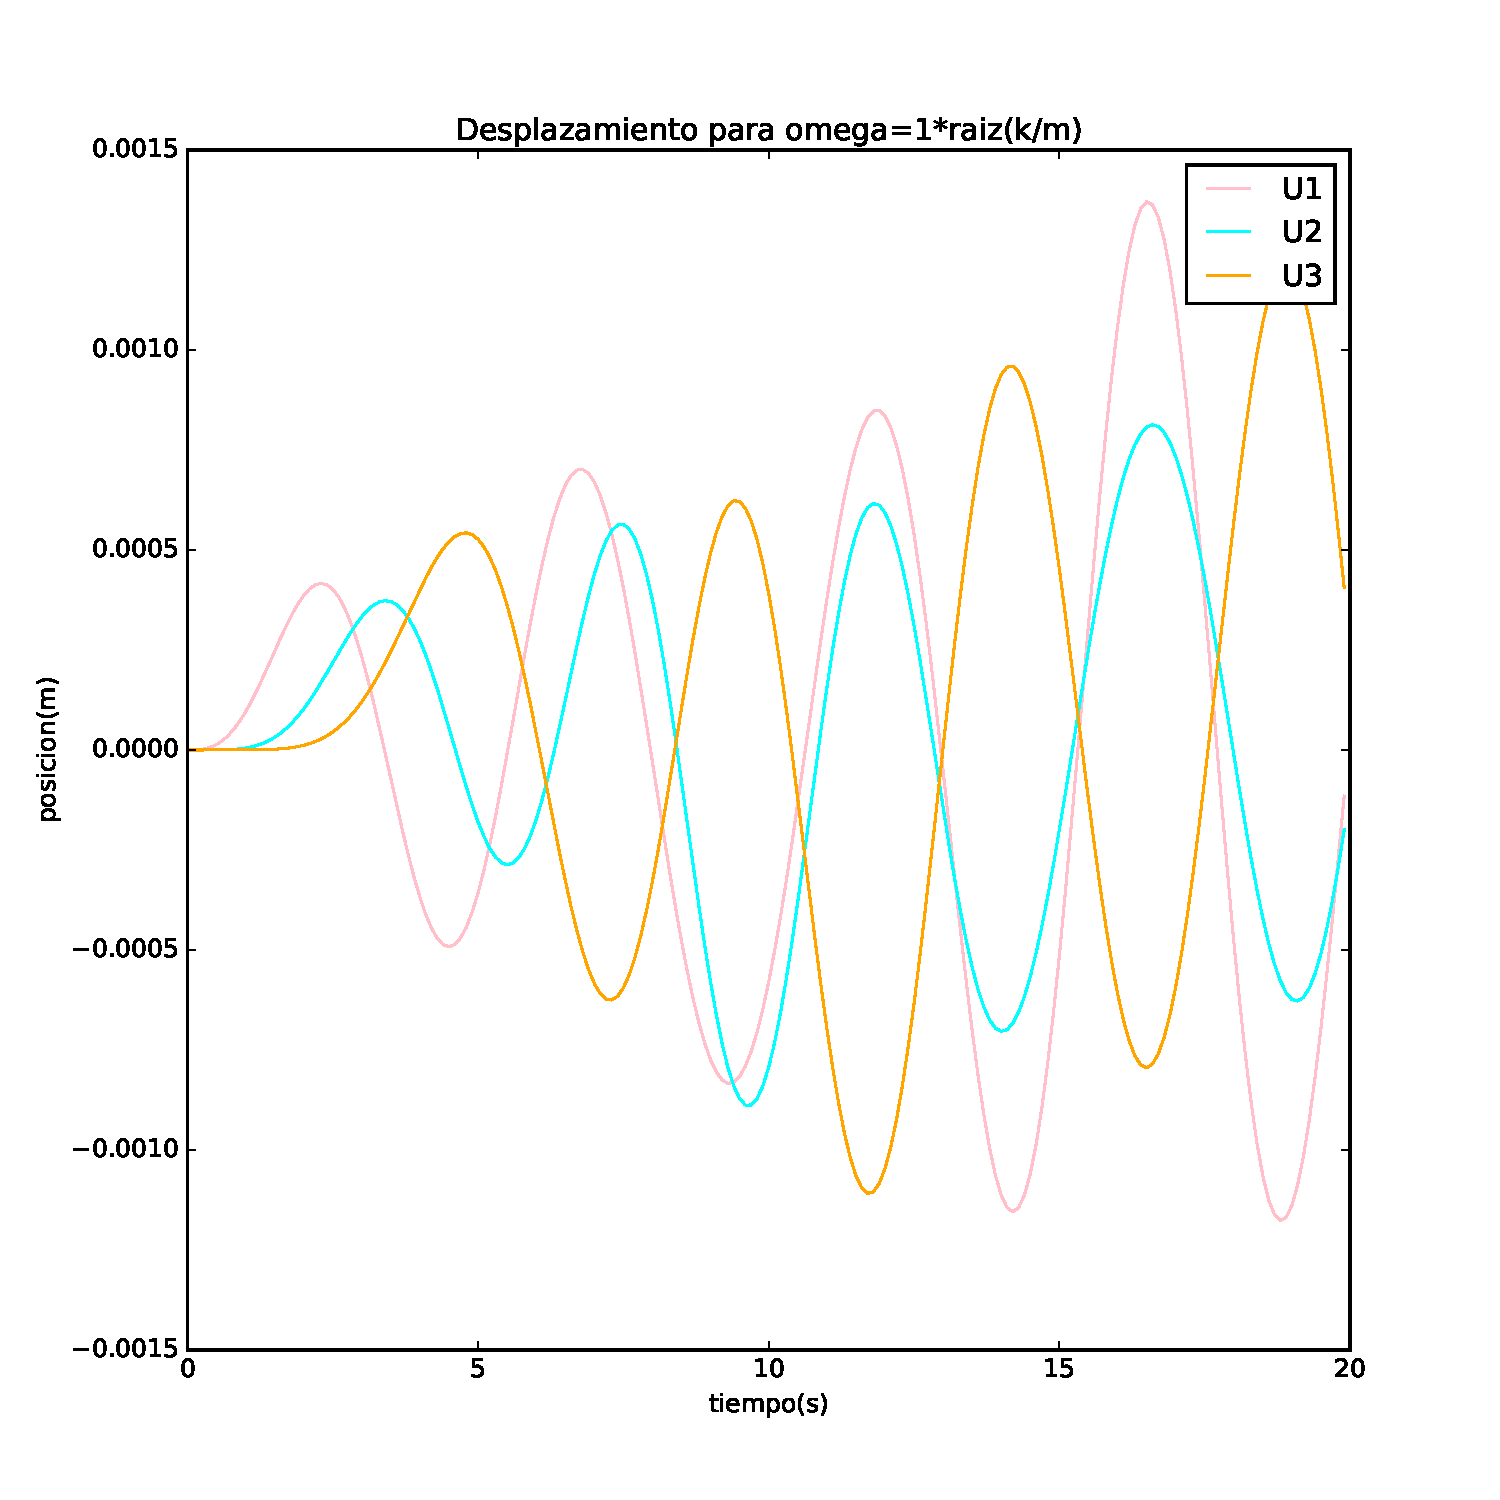
\includegraphics[width=1\textwidth]{plot_omegafijo.pdf}
    \caption{Desplazamiento del edificio en el tiempo}
    \label{fig:my_label}
\end{figure}
Esta grafica se obtuvo para el primer omega, se tiene que una vez el primer piso se desplaza los otros dos pisos comienzan a desplazarse con cierto desfase. Se observa que la amplitud del movimiento del edificio aumenta con el pasar del tiempo y que muchas veces el tercer y el primer piso tienen desplazamientos completamente contrarios. Esto nos indica que los edificios deben tener cierta elasticidad para poder soportar el movimiento ondulatorio que se genera a partir de los temblores. 
\subsection{Grafica de las mayores amplitudes para cada uno de los 100 omegas generados}
\begin{figure}[H]
    \centering
    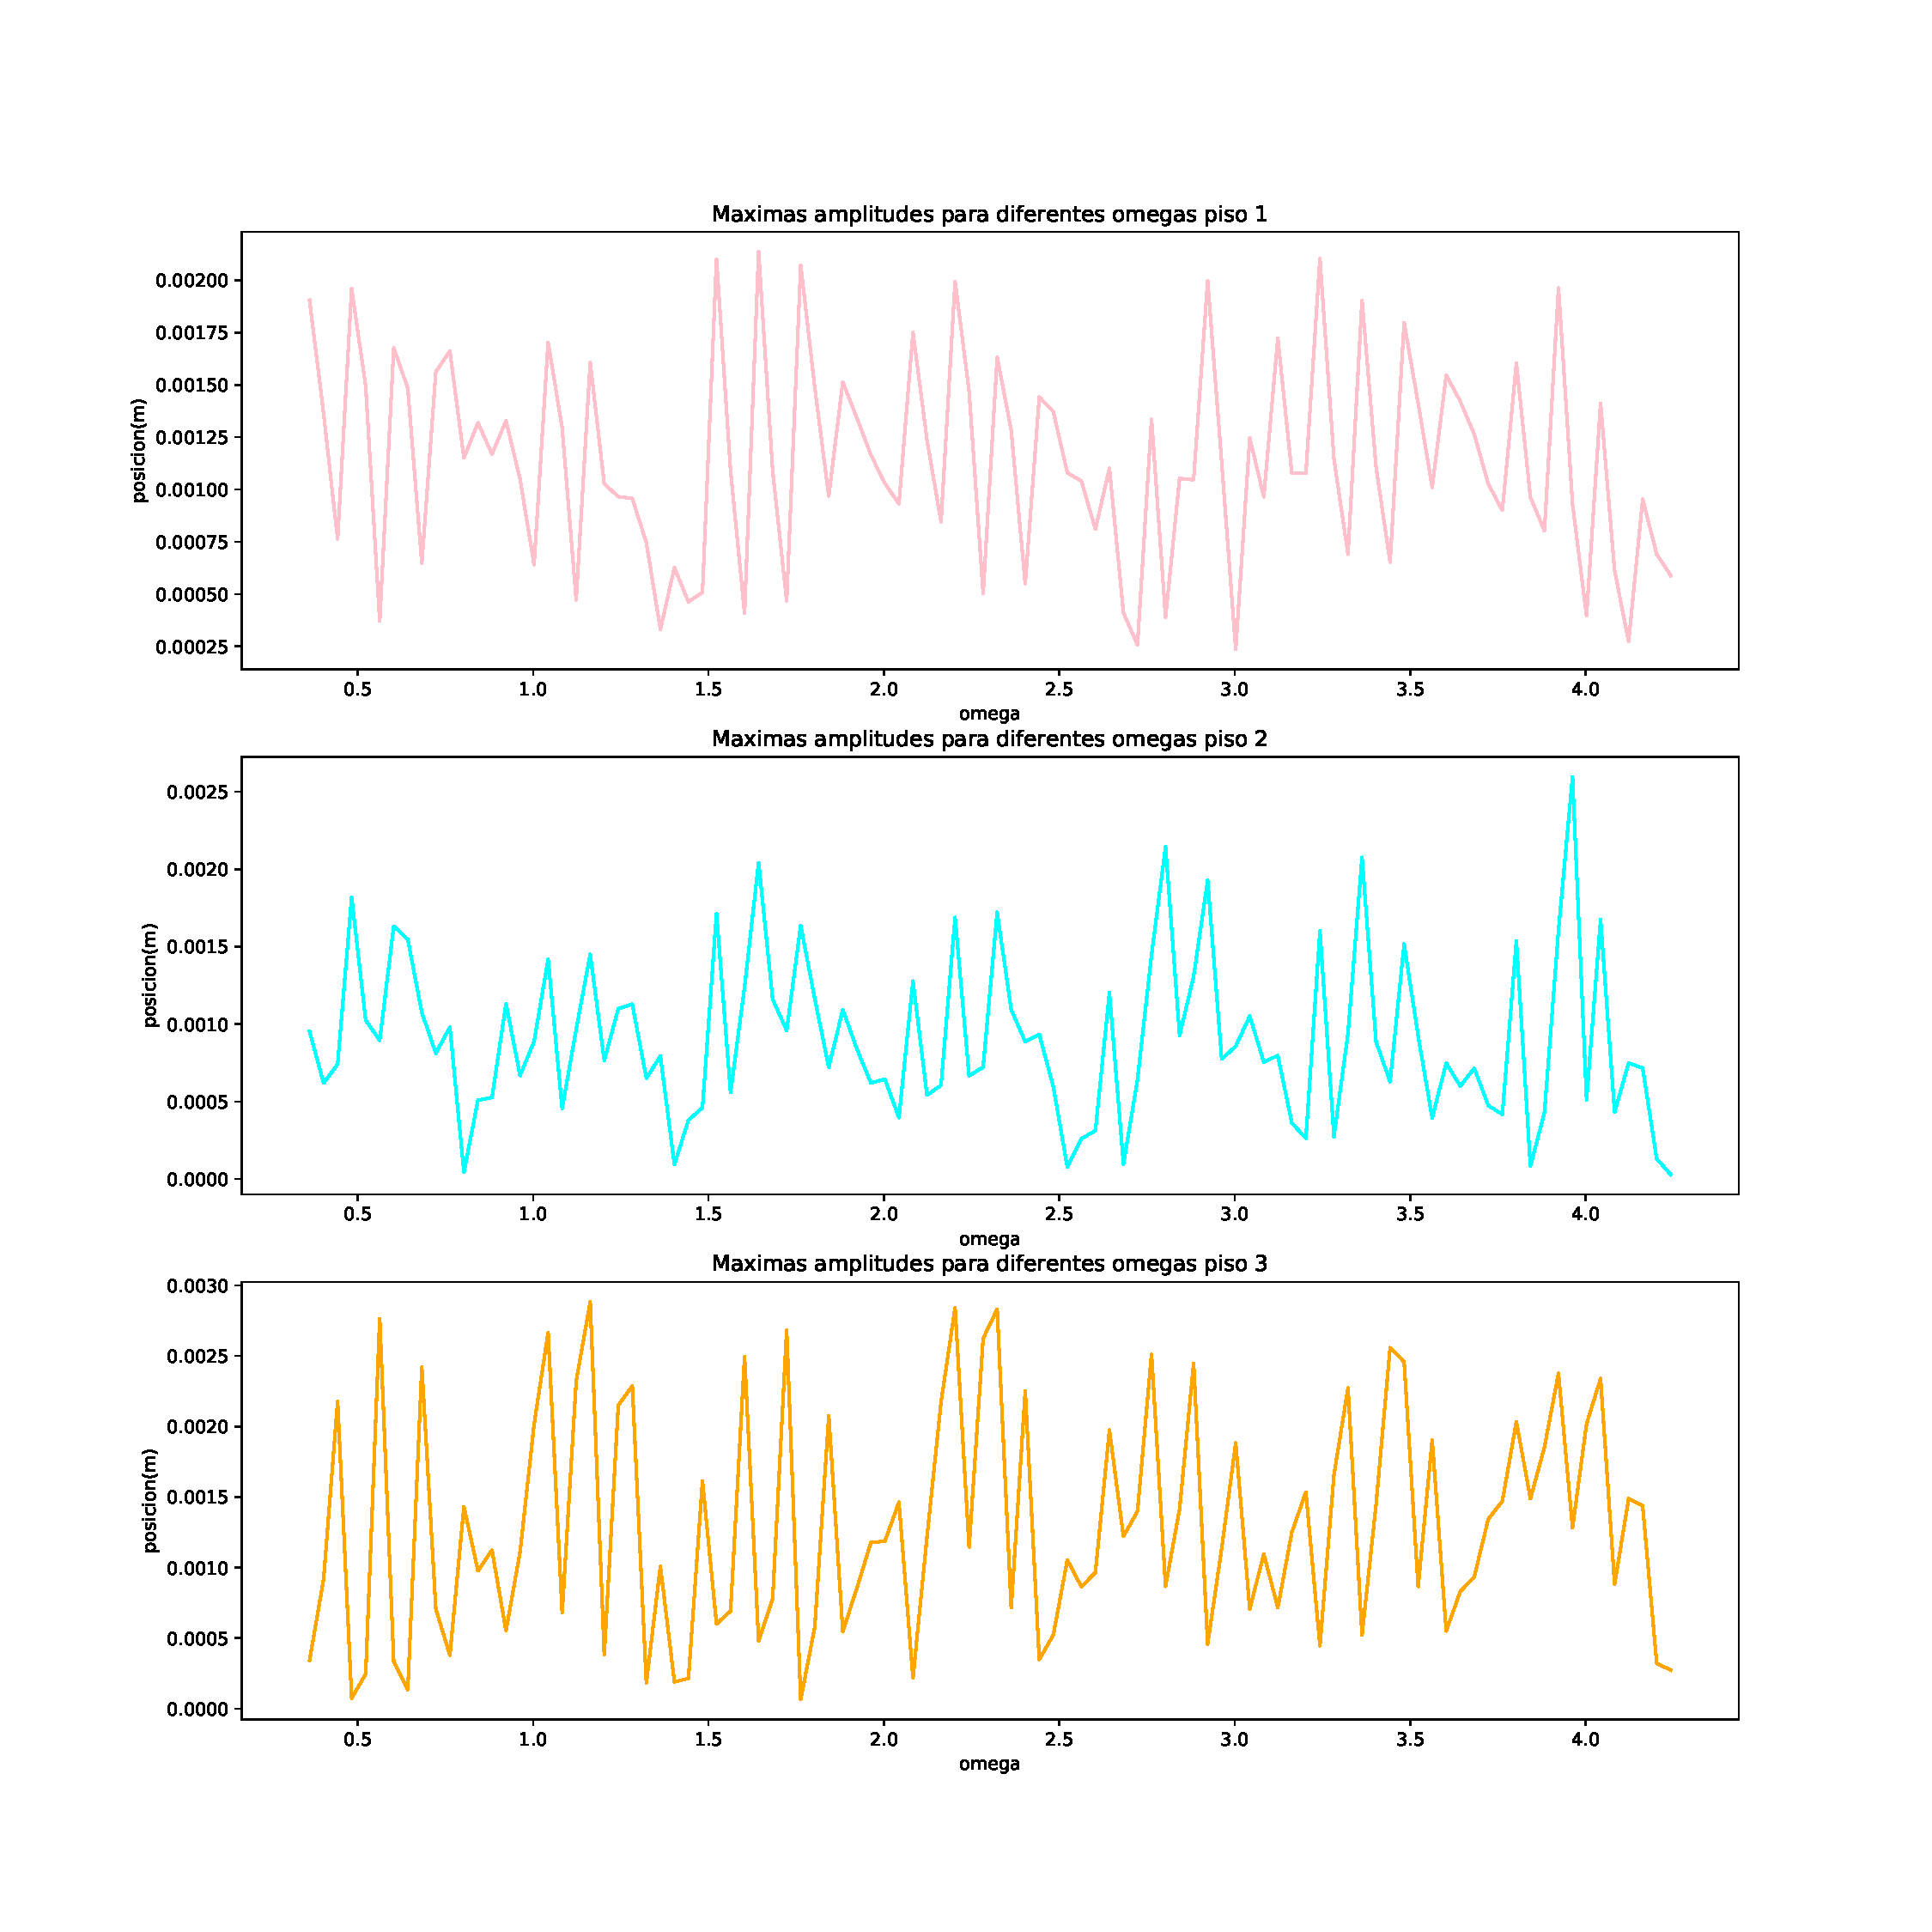
\includegraphics[width=1\textwidth]{plot_omegas.pdf}
    \caption{Mayores amplitudes para cada omega}
    \label{fig:my_label}
\end{figure}

Lo anterior se hizo 100 veces para 100 omegas diferentes y se obtuvo la grafica de la figura 8. De esta se obtiene que un sistema de tres masas no tiene una sola frecuencia de resonancia sino varias. En general, hay aproximadamente 13 picos por piso. Esta grafica nos permitio hacer otras cuatro graficas variando los omegas, ya que nos permitio escoger omegas que dan amplitudes interesantes. 
\subsection{Grafica de los cuatro omegas}
Los omegas se escogieron al revisar la figura 8.
Estos omegas se pueden revisar tanto en Plotshw2.py como en Edificio.cpp. 
\begin{figure}[H]
    \centering
    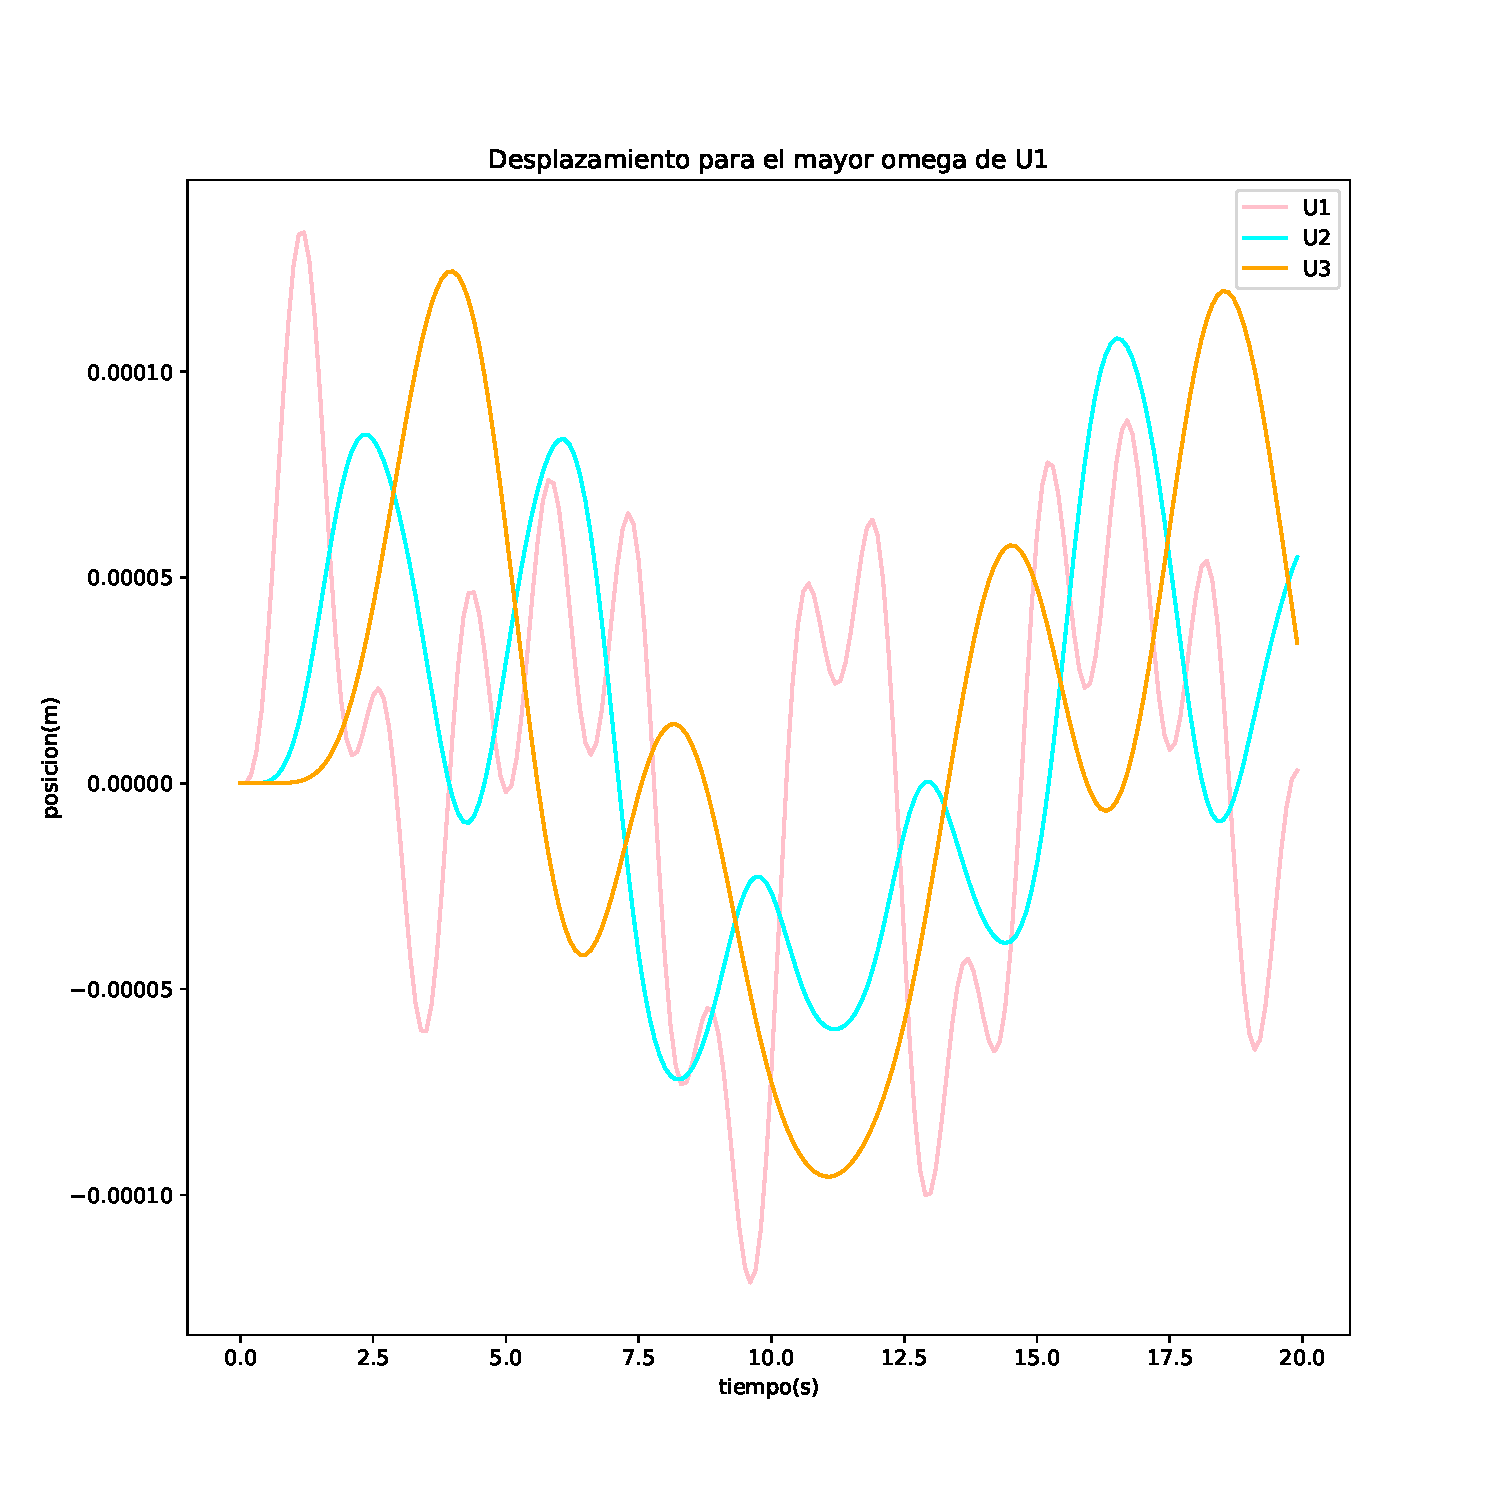
\includegraphics[width=1\textwidth]{plot_omega1.pdf}
    \caption{ Desplazamiento para omega=3.72267}
    \label{fig:my_label}
\end{figure}
Al tener un omega muy alto, la velocidad del primer piso y las posiciones del primer piso cambian mucho mas que las de los otros dos pisos. Se observa que la amplitud no es tan alta en este caso. Esto se debe a la rapidez del primer piso, que frena de cierta forma la de los otros dos pisos.
\begin{figure}[H]
    \centering
    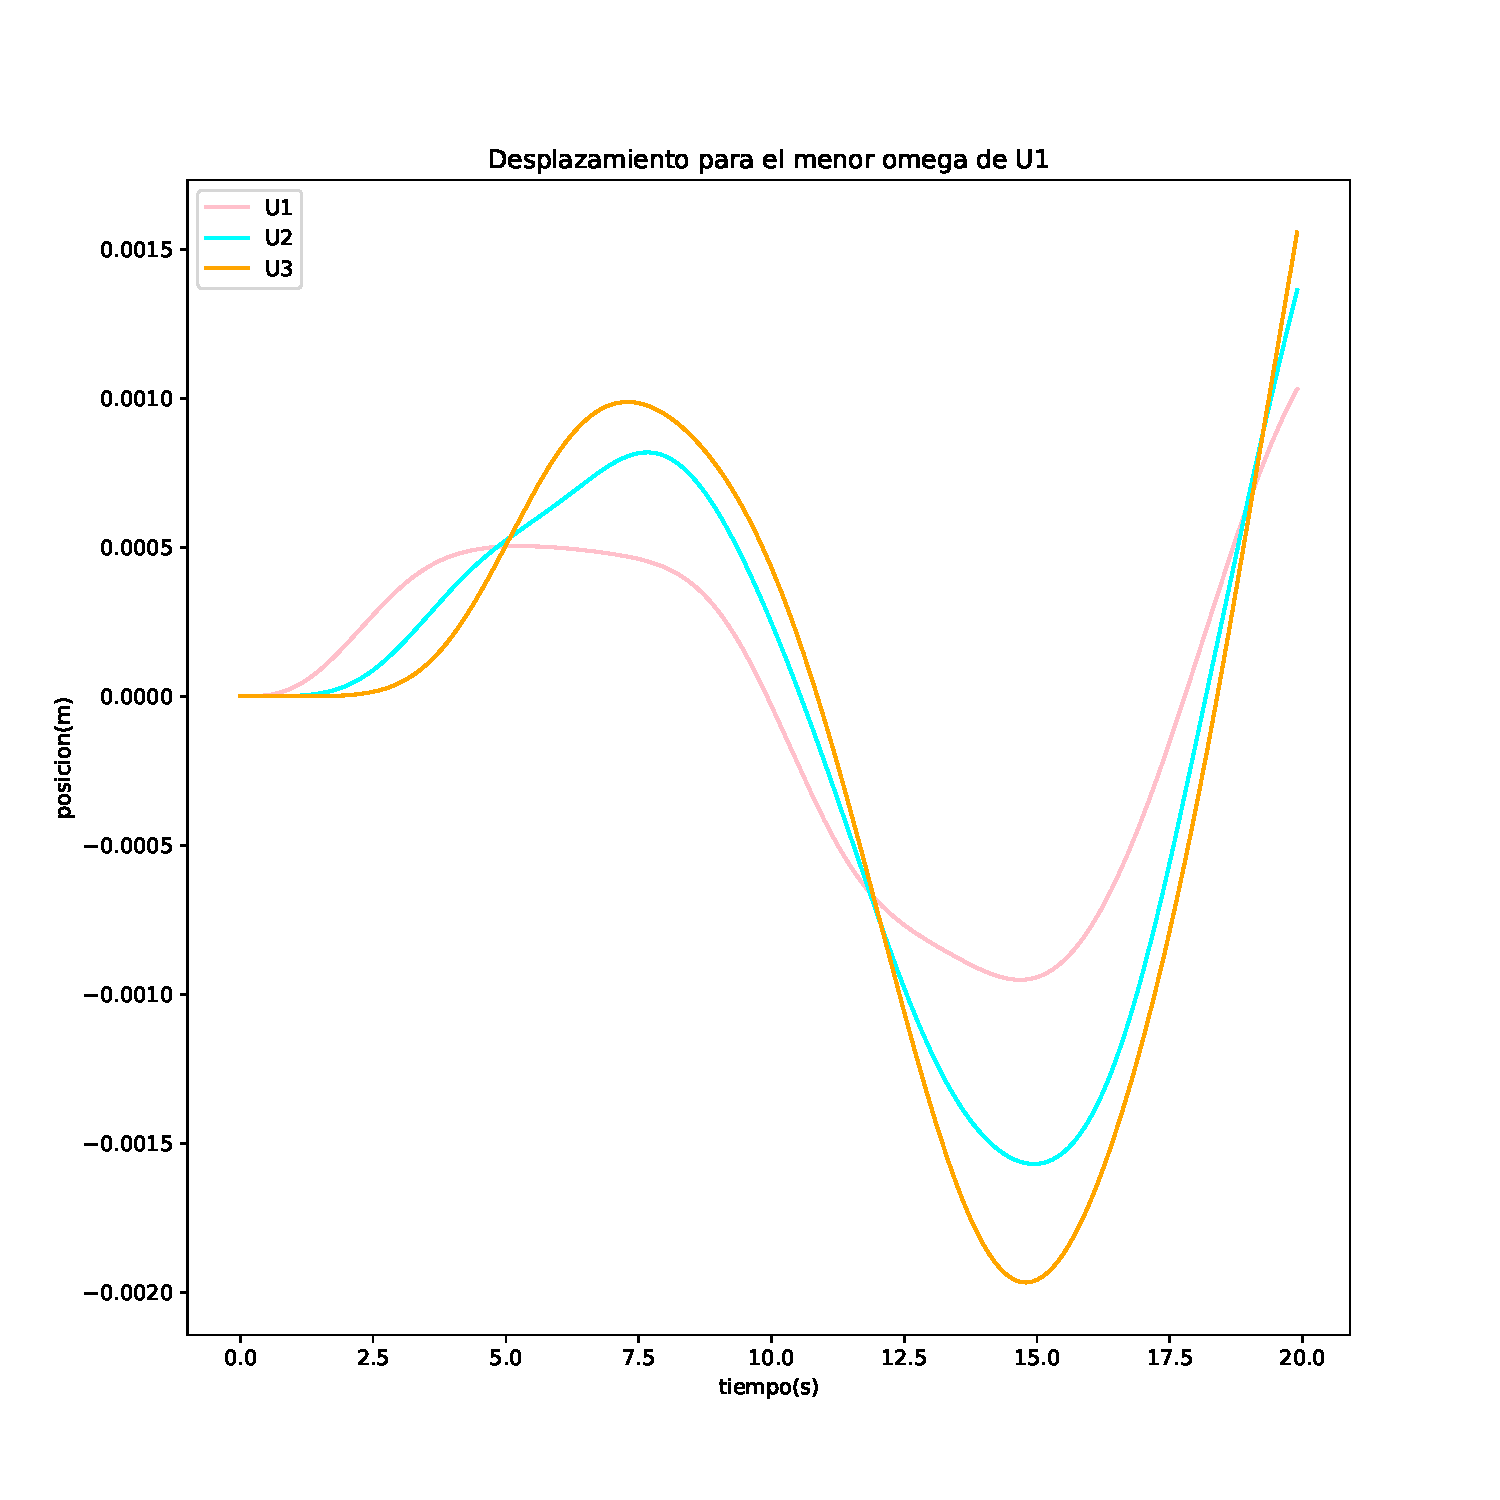
\includegraphics[width=1\textwidth]{plot_omega2.pdf}
    \caption{ Desplazamiento para omega=0.402837}
    \label{fig:my_label}
\end{figure}
Al tener un omega muy pequenio, la velocidad del primer piso y las posiciones del primer piso cambian mucho menos que las de los otros dos pisos. Se observa que la amplitud es muy alta en este caso. Esto no indica que estamos acercandonos a la frecuencia de resonancia y que para omegas pequenios hay mas probabilidades de que el edificio se caiga. En este caso no se ve el desfase, el edificio no se mueve como un sistema de tres masas sino bastante parecido al sistema de una sola masa. 
\begin{figure}[H]
    \centering
    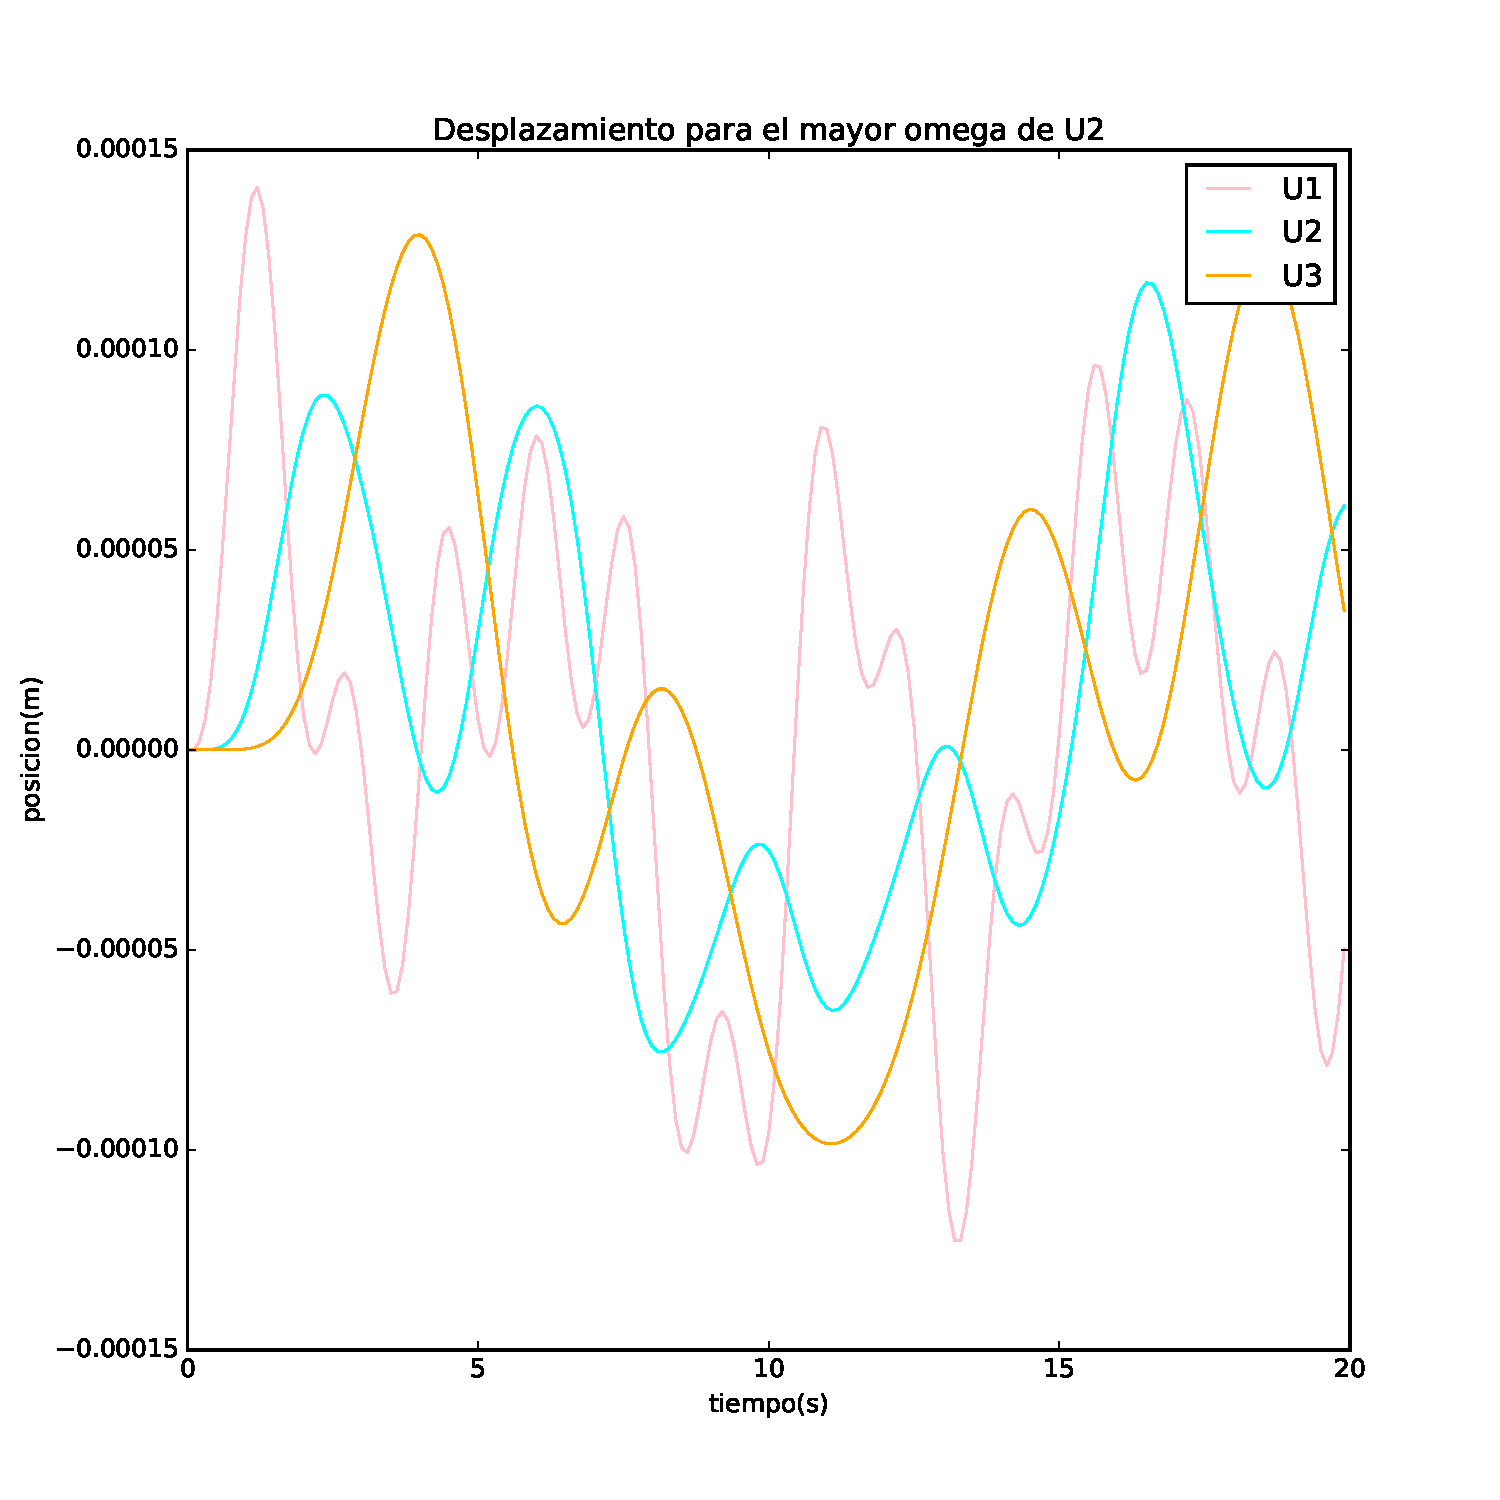
\includegraphics[width=1\textwidth]{plot_omega3.pdf}
    \caption{Desplazamiento para omega=3.92266}
    \label{fig:my_label}
\end{figure}
En este caso se observa algo muy similar a lo visto en la figura 9. Al tener un omega muy alto, la velocidad del primer piso y las posiciones del primer piso cambian mucho mas que las de los otros dos pisos. Se observa que la amplitud no es tan alta en este caso. Esto se debe a la rapidez del primer piso, que frena de cierta forma la de los otros dos pisos.
\begin{figure}[H]
    \centering
    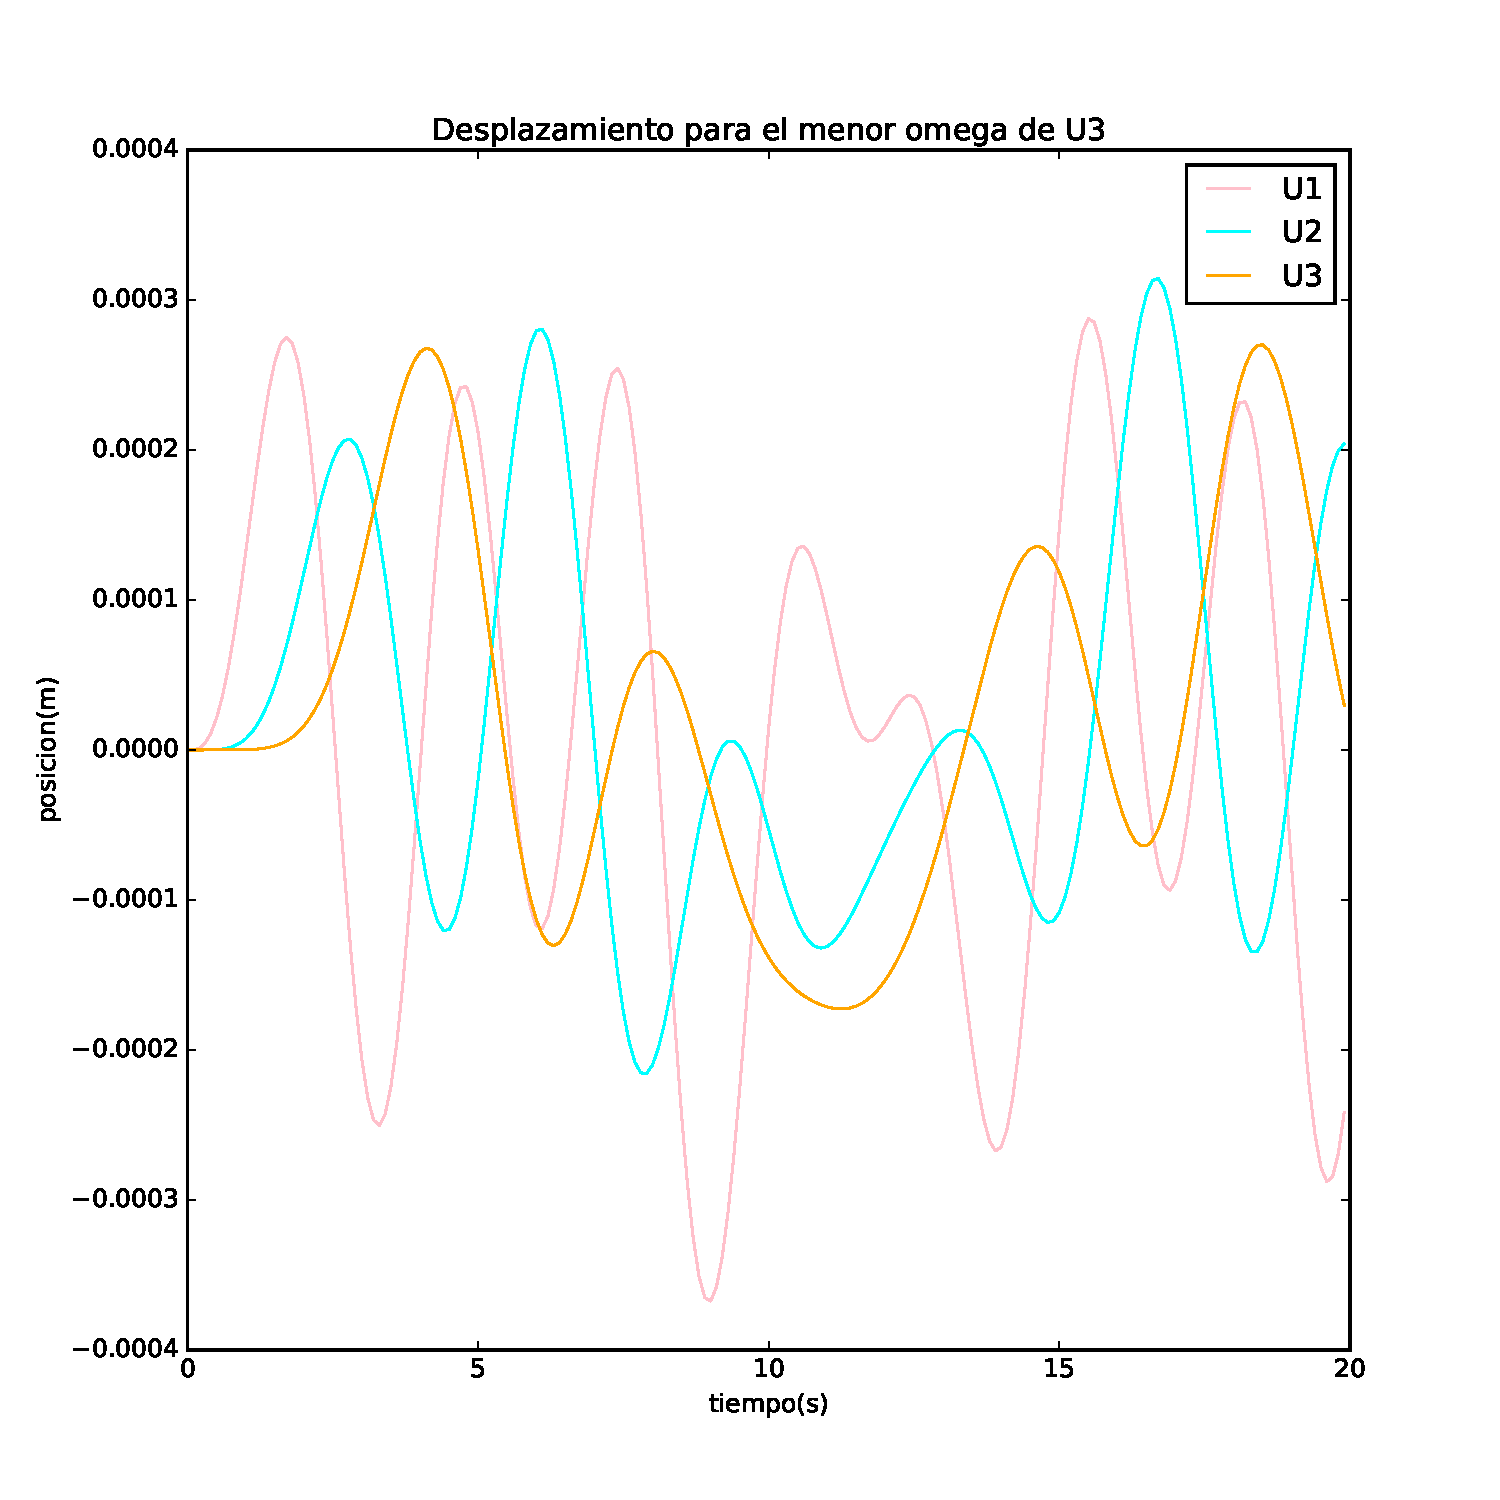
\includegraphics[width=1\textwidth]{plot_omega4.pdf}
    \caption{Desplazamiento para omega=2.32274}
    \label{fig:my_label}
\end{figure}
En este caso se observa algo muy similar a lo visto en la figura 9. Sin embargo, con este omega se alcanzan amplitudes superiores. Una vez mas, se ve que la posicion del primer piso cambia mucho mas que la de los otros dos pisos. 
\subsection{Bono}
\subsubsection{Cambio en las masas de los pisos}
\begin{figure}[H]
    \centering
    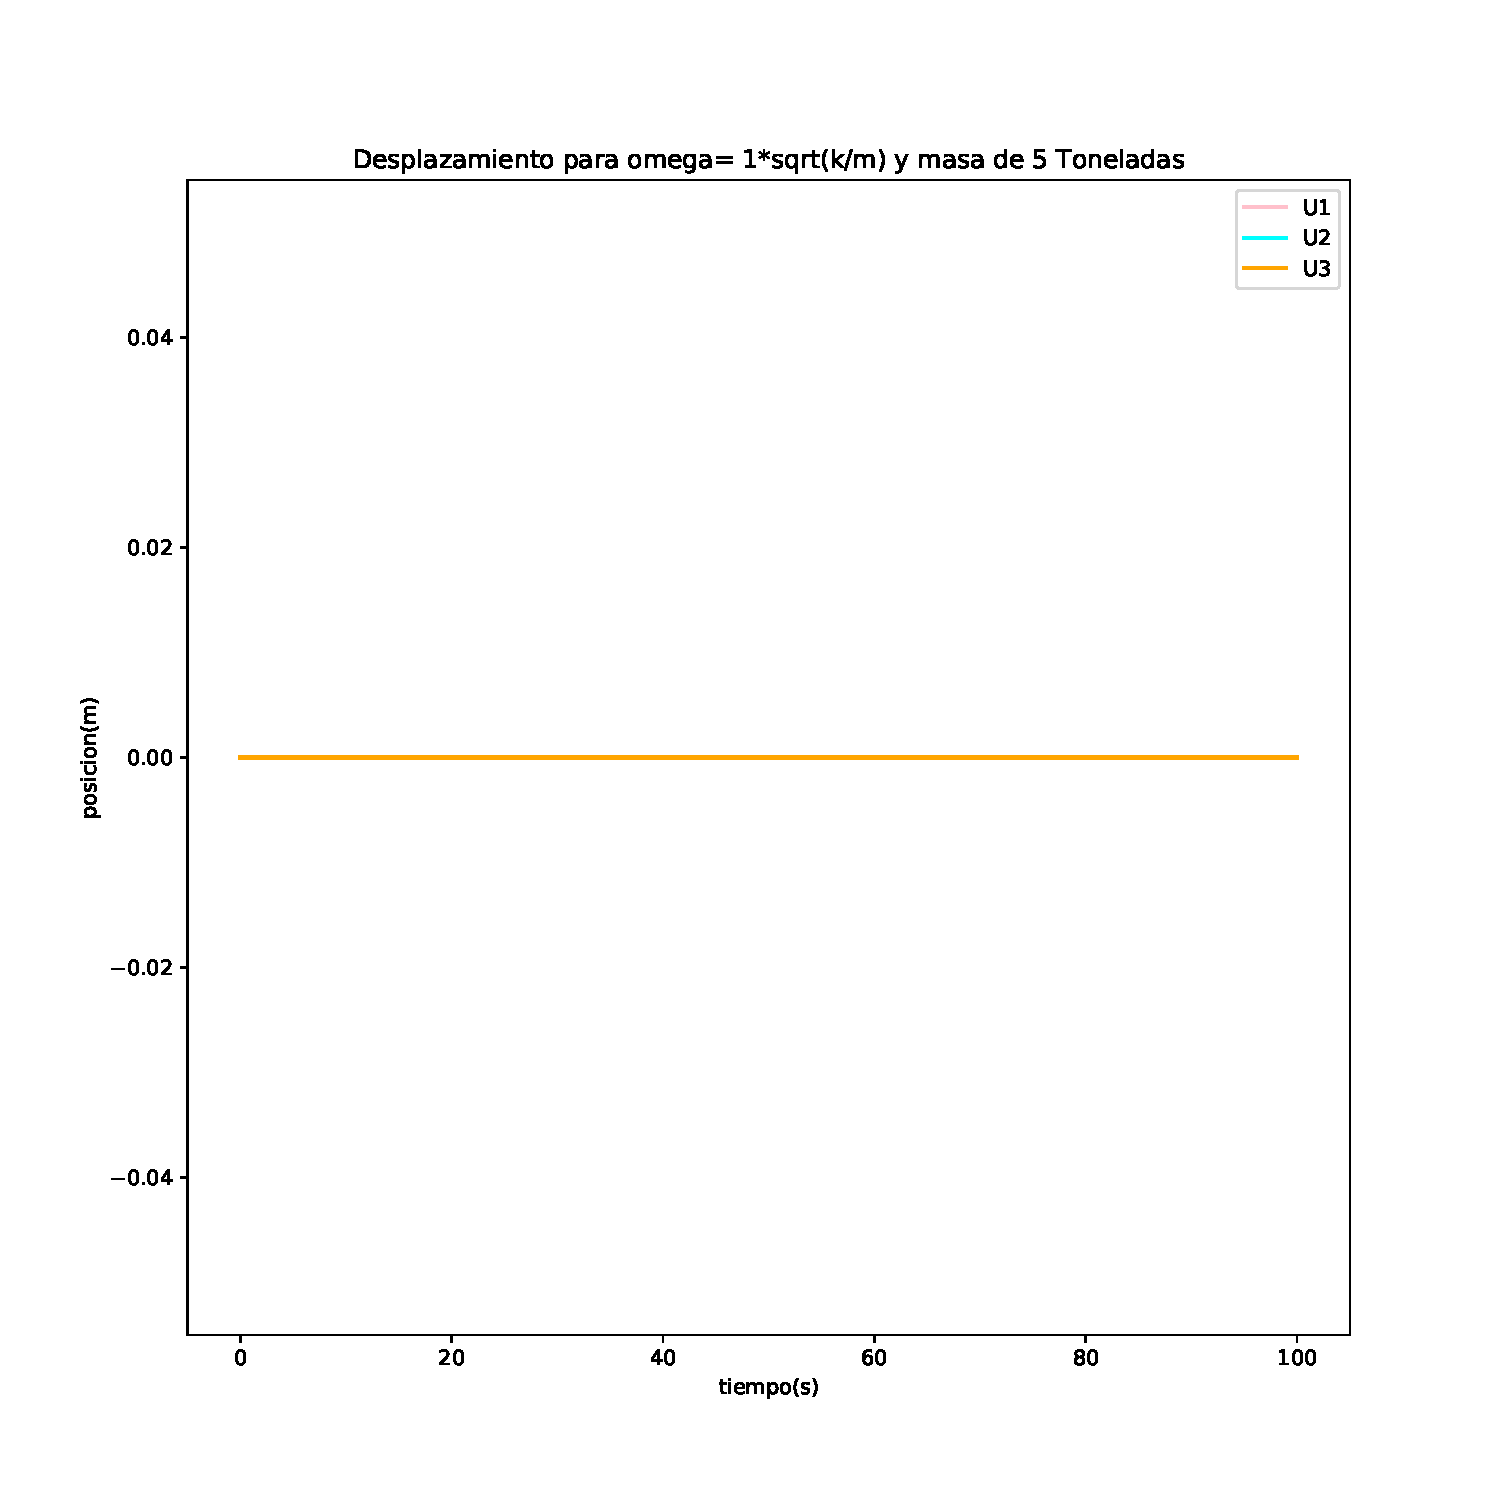
\includegraphics[width=1\textwidth]{masas.pdf}
    \caption{Desplazamiento para una masa de 5000kg}
    \label{fig:my_label}
\end{figure}
En esta grafica se observa que si la masa del edificio aumenta el desplazamiento es nulo. Esto tiene sentido ya que es mucho mas dificil mover algo muy pesado. Ademas, las ecuaciones dependen del forzamiento en el primer paso y dada la formulacion de este, un masa muy grande hace que todo tienda a cero y que no se pueda estudiar el diferentes masas con las ecuaciones planteadas. 
\begin{figure}[H]
    \centering
    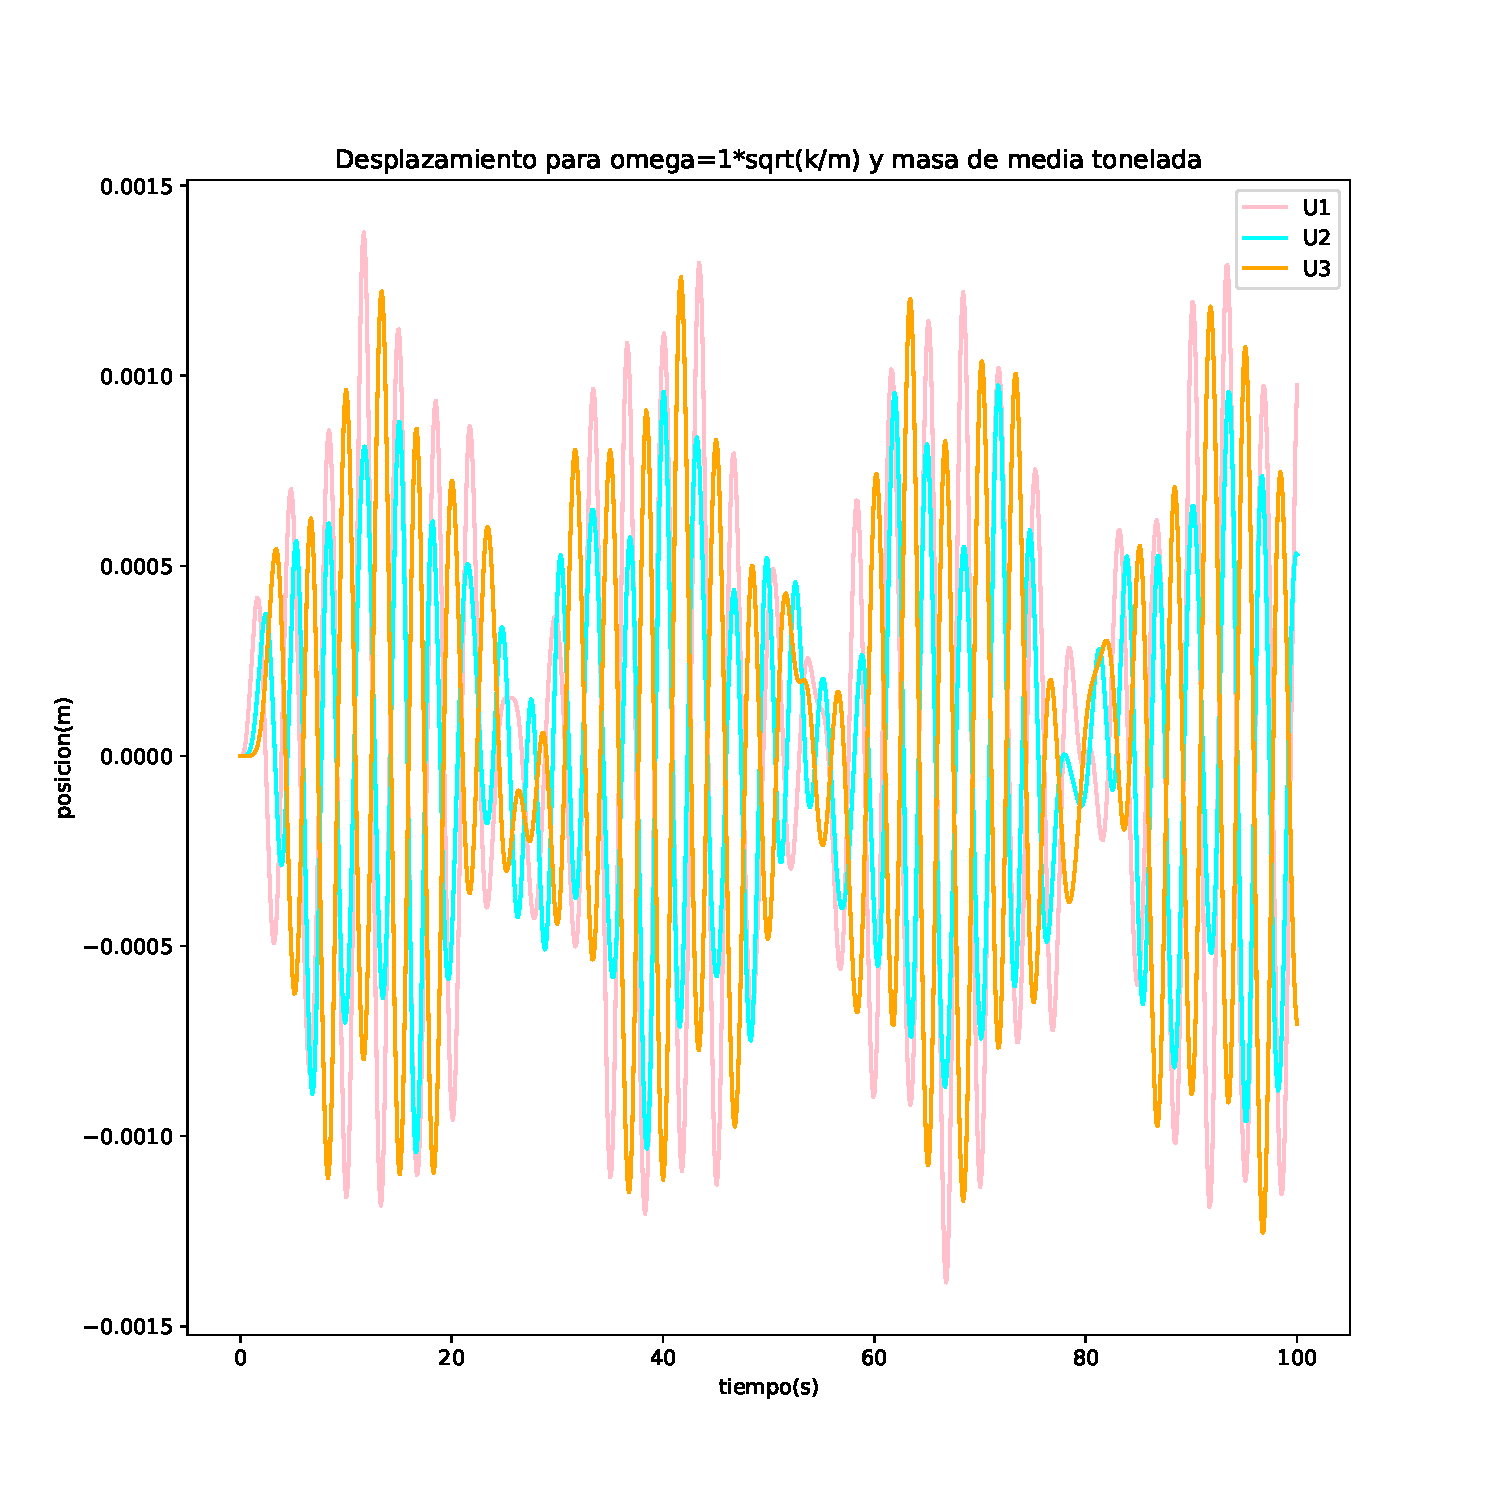
\includegraphics[width=1\textwidth]{masas1.pdf}
    \caption{Desplazamiento para una masa de media toneladas}
    \label{fig:my_label}
\end{figure}
En esta grafica se tiene que la masa es 500 kg y se ve un desplazamiento bastante particular. En efecto el periodo disminuye bastante. Se observa que el desplazamiento se va a cero repetidas veces. Las amplitudes no cambian. 
\begin{figure}[H]
    \centering
    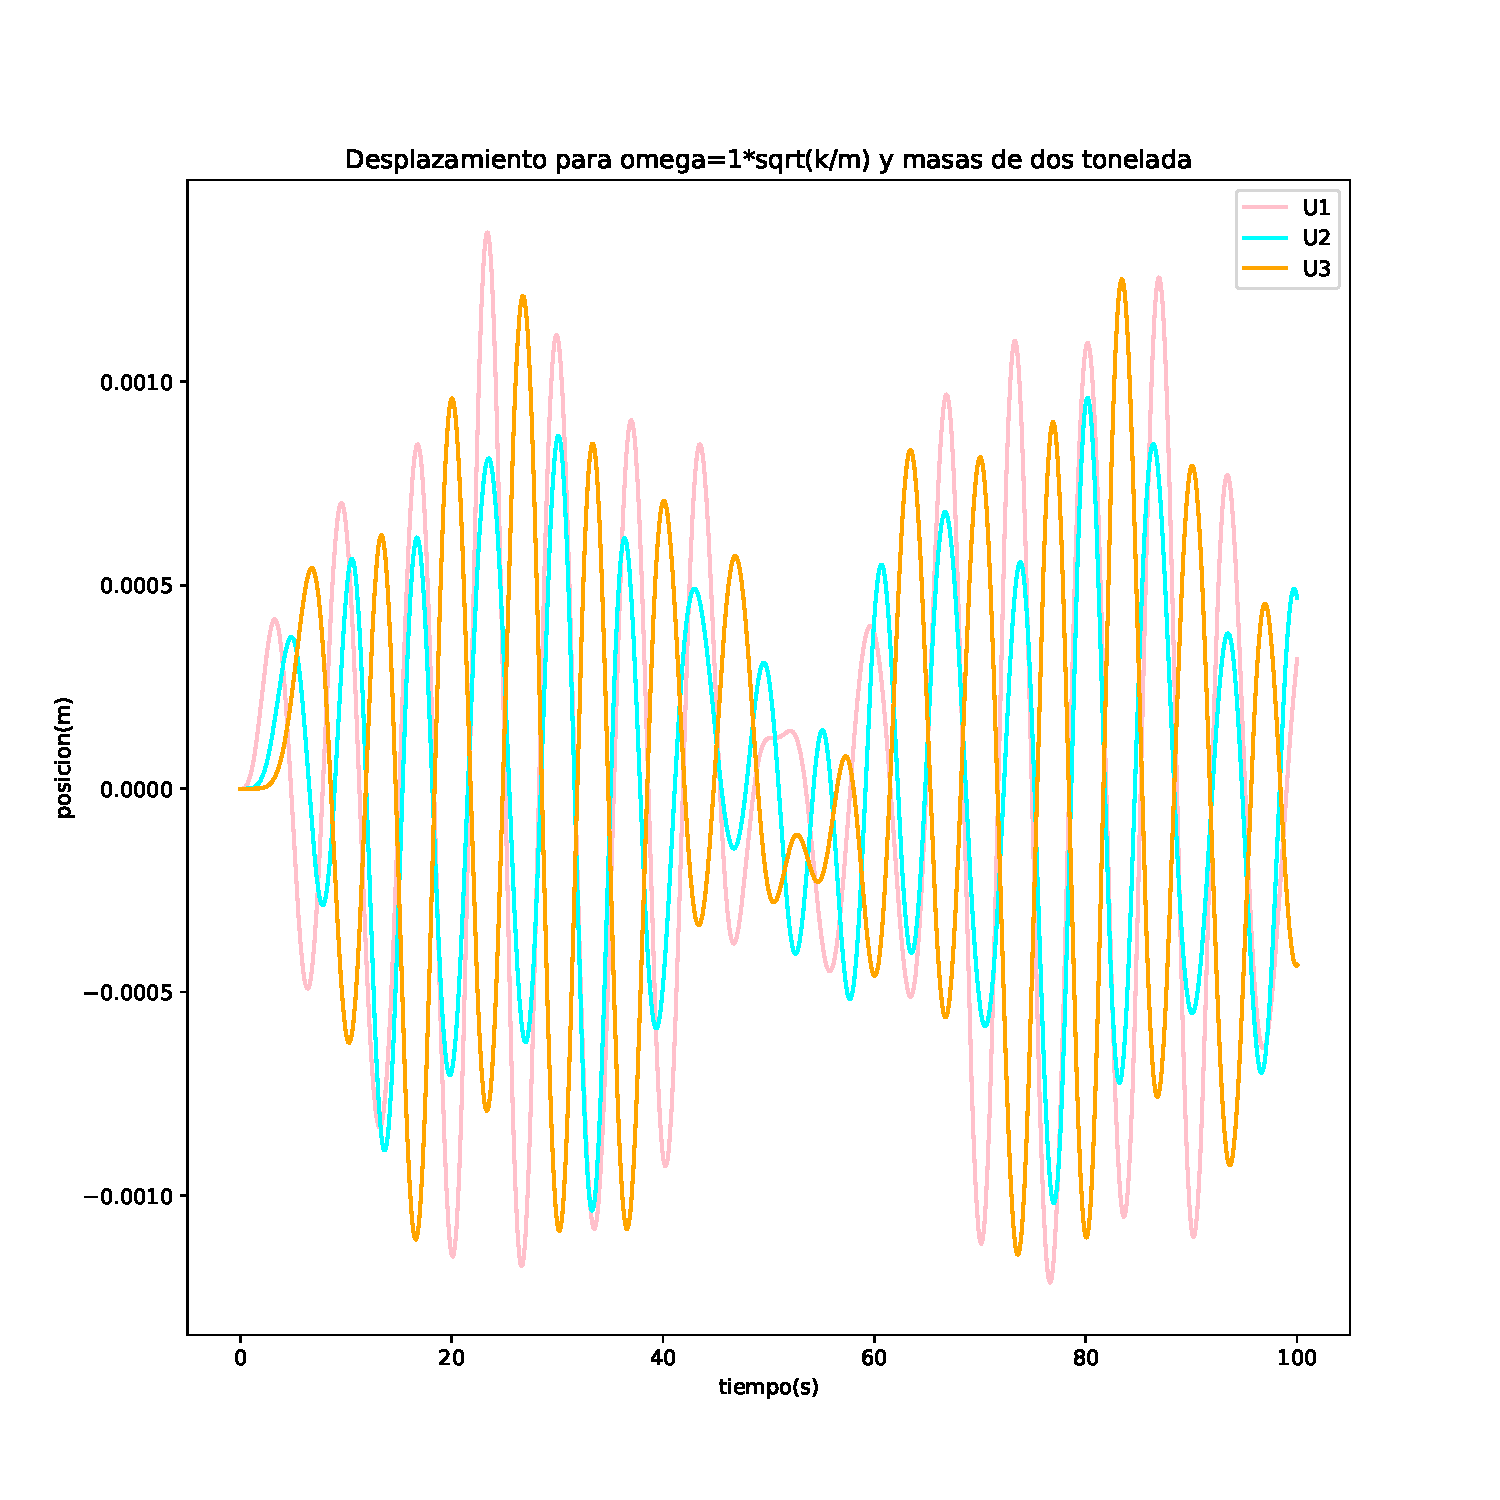
\includegraphics[width=1\textwidth]{masas2.pdf}
    \caption{Desplazamiento para una masa de dos toneladas}
    \label{fig:my_label}
\end{figure}
En esta grafica se observa el caso en el que masa y la constante K son iguales, por lo que omega es igual a 1. Se observa que el periodo aumento y que el despalazamiento tampoco cambia mucho. Por lo tanto las masas no cambian mucho el desplazamiento si varian ligeramente pero siempre cambian en periodo. 
\subsubsection{Gammas realistas}
Los gammas utilizados en este ejercicio fueron sacados del siguiente link \url{https://www.finesoftware.es/ayuda-en-linea/geo5/es/tabla-de-factores-de-friccion-de-diferentes-materiales-01/}. Se hizo un promedio y se determino que el coeficiente de friccion seria 0.41. 
\begin{figure}[H]
    \centering
    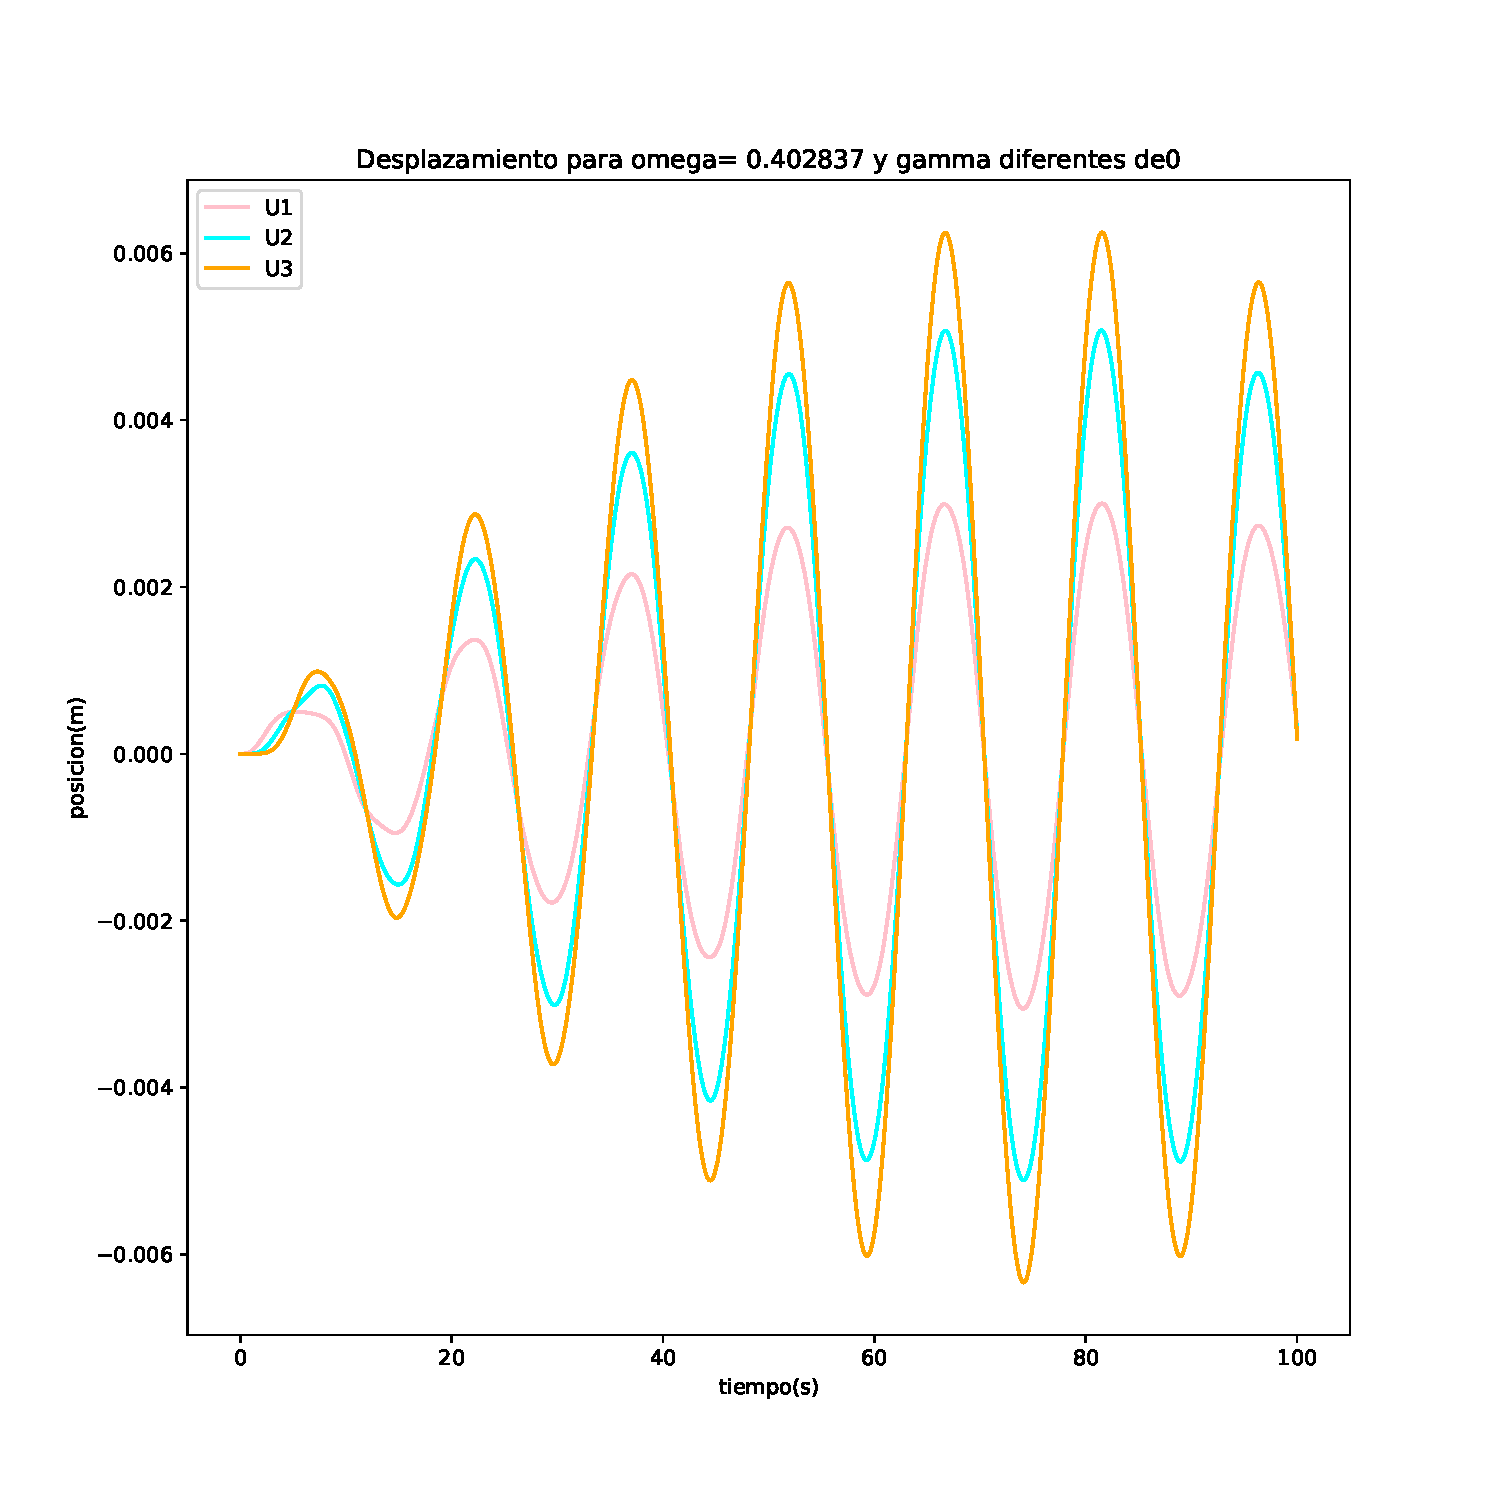
\includegraphics[width=1\textwidth]{gammas.pdf}
    \caption{Desplazamiento para omega=0.402837}
    \label{fig:my_label}
\end{figure}
Para esto se utilizo el mismo omega que en la figura 10 y se observa que el desplazamiento de todos los pisos disminuyo y que al aniadir un coeficiente de friccion entre los pisos y el suelo ya no se ve un desfase en los movimientos de los pisos. En efecto, este coeficiente hace que el edificio se comporte como una masa sola en vez de tres diferentes conectadas. 
\begin{figure}[H]
    \centering
    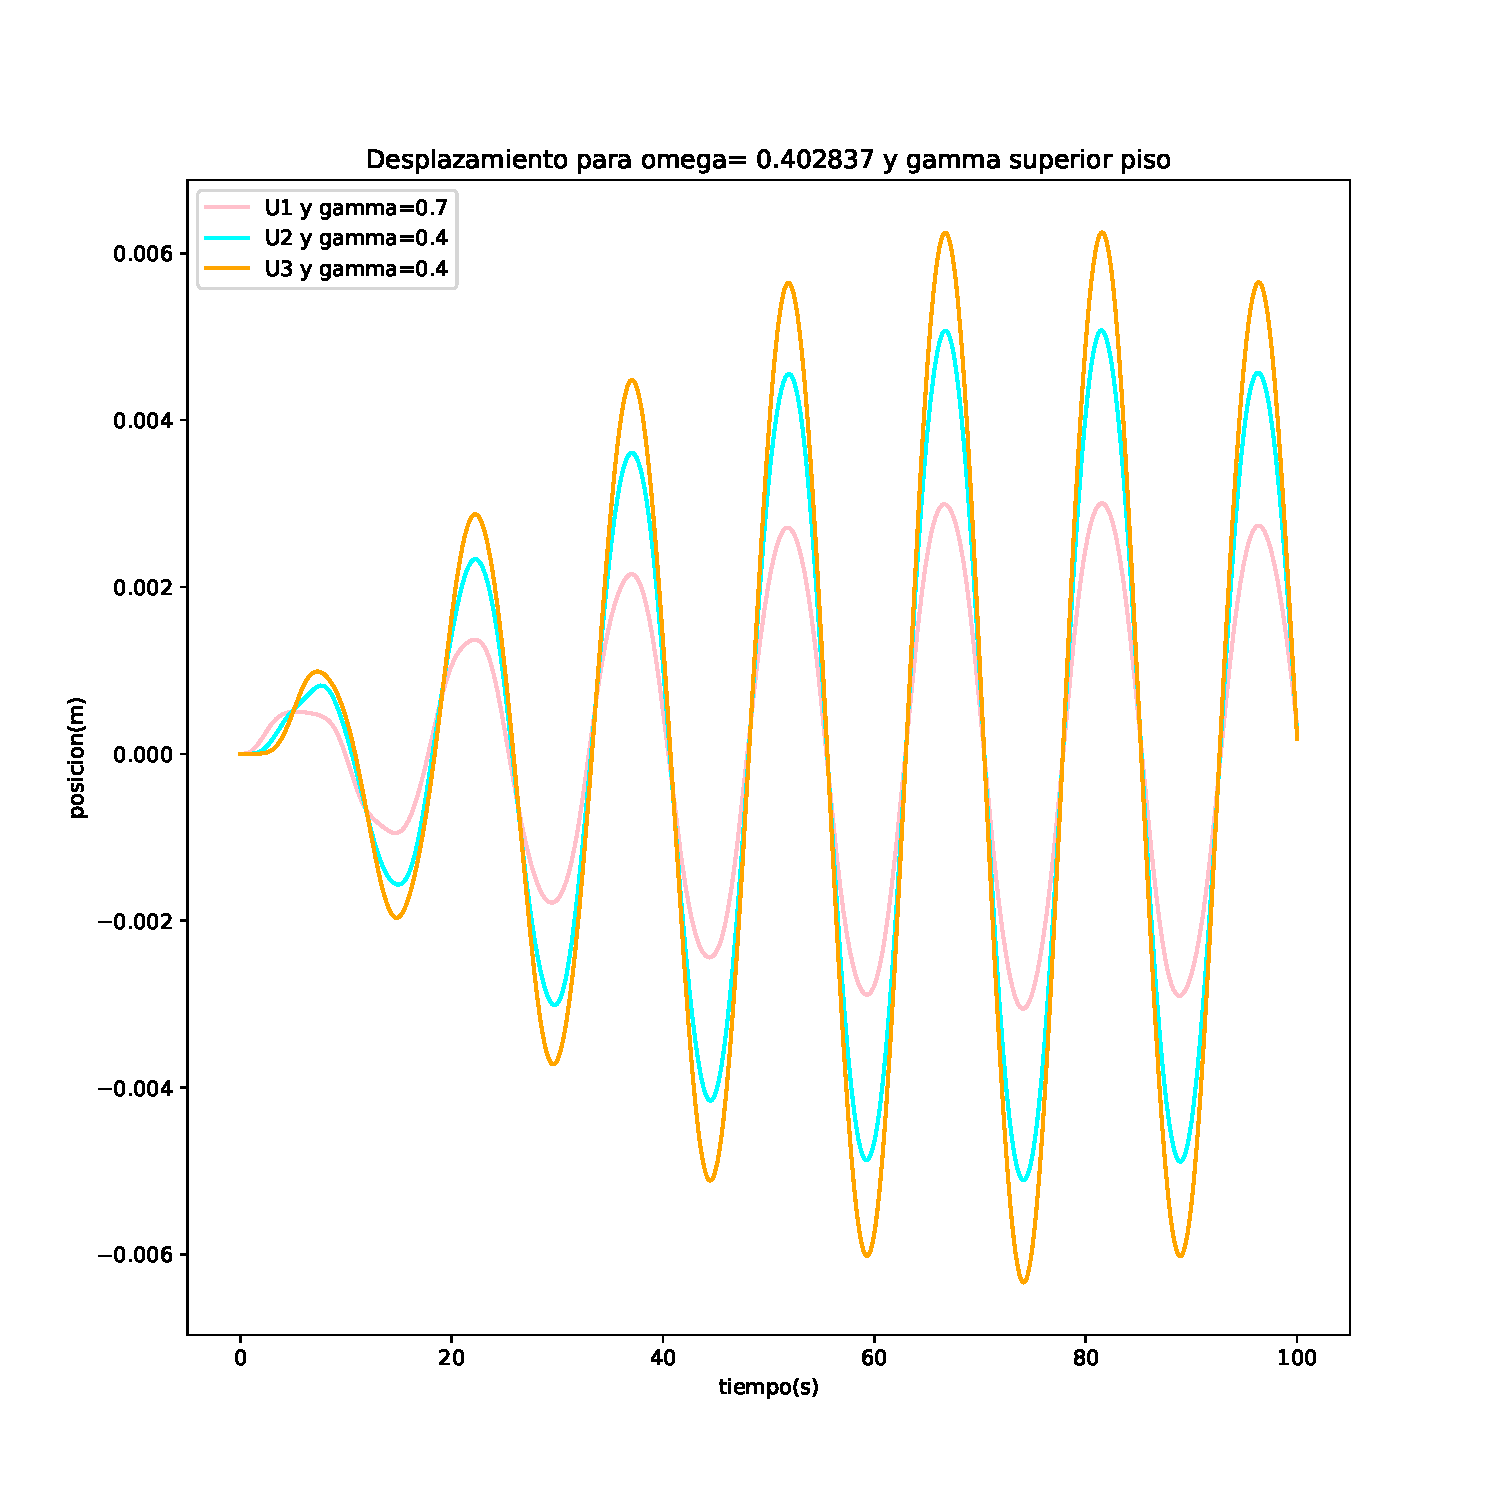
\includegraphics[width=1\textwidth]{gammas1.pdf}
    \caption{Desplazamiento para omega=0.402837}
    \label{fig:my_label}
\end{figure}
Para esta figura se decidio cambiar el coeficiente de friccion del primer piso con respecto al suelo a 0.7, ya que es el valor realista posible mas grande. Se decidio dejar u coeficiente de friccion de 0.4 para los otros pisos. Como se observa en la grafica no hay mayor cambio, esto se puede observar en las ecuaciones, ya que la friccion no tiene un coeficiente muy importante. 
Por  otro lado, se tiene que entre mayor la friccion, menor la flexibilidad del edificio y mayor posibilidades de accidentes. 
\begin{figure}[H]
    \centering
    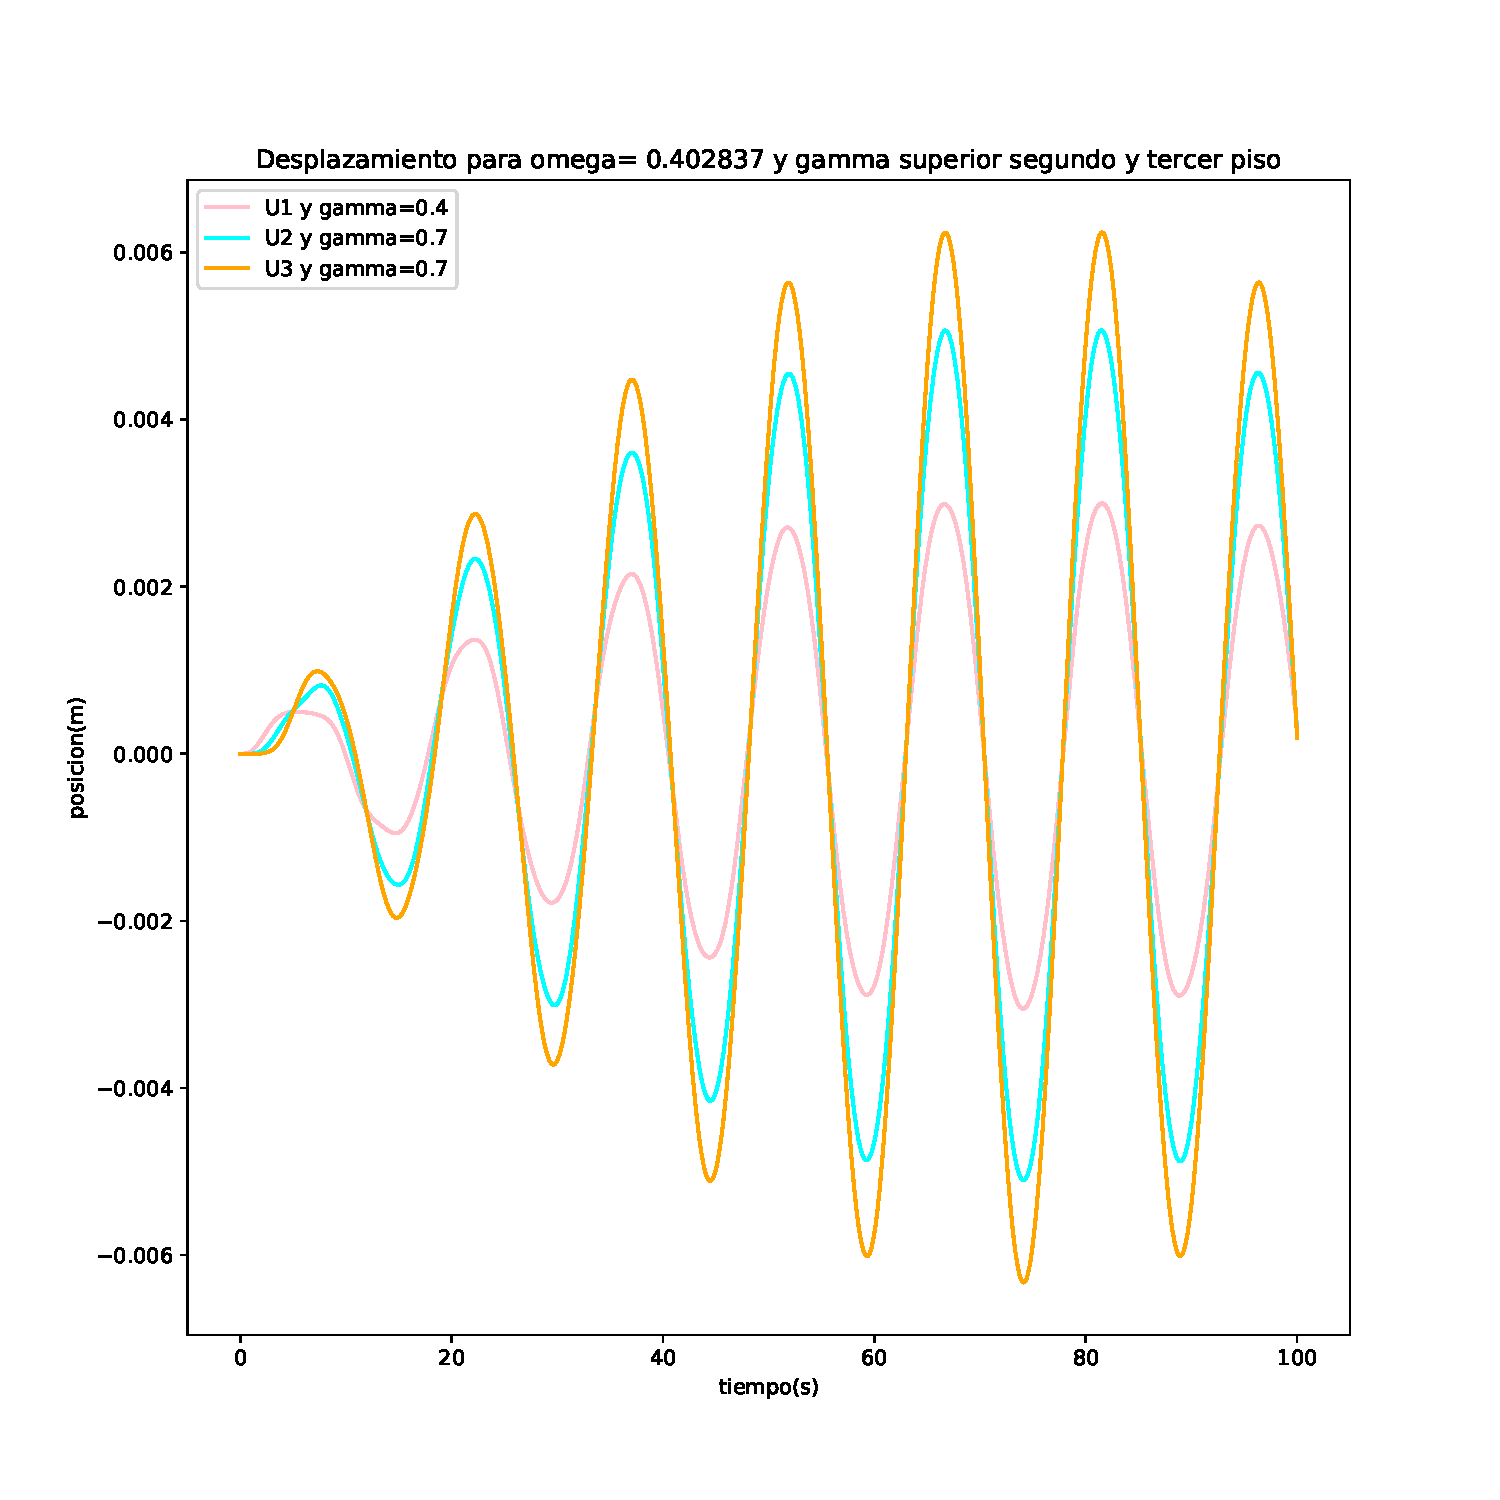
\includegraphics[width=1\textwidth]{gammas2.pdf}
    \caption{Desplazamiento para omega=0.402837}
    \label{fig:my_label}
\end{figure}
En esta grafica se trato de cambiar los coeficientes de forma inversa a lo visto en la grafica anterior. Las conclusiones son las mismas que la grafica anterior. 
\end{document}